%!TeX program=pdflatex
%!TeX encoding=utf8
%!TeX spellcheck = en_US
%!TeX root = ../../messageVortex.tex


% ********************************************************************************************************
% *** Methodes
% ********************************************************************************************************
\part{Methodes\label{sec:methodes}}
In this part of the thesis, we collect requirements, definitions, methods, and existing research relevant to the topic of this thesis. We explain the choices made and what solutions have been discarded.

We start by collecting requirements for the protocol. Having the requirements, we collect existing technologies on research and implementation levels. Each of the techniques is quickly categorized and either further studied or rejected, naming the reasons for rejection.

The list of technologies and research collected is big. All relevant technologies, either widely adopted or thoroughly researched, should be included in this chapter. All Technologies and research are categorized. We reference technologies through their standards. If applicable, multiple standards may be part of the analysis. A short introduction into the protocol is given and then analyzed for suitability for a specific problem addressed in this work. Whenever quoting research, we refer to the respective papers. If appropriate, multiple related pieces of research are collected together into a bigger picture and then analyzed. When analyzing, we focus on suitability concerning specific problems. If related to standard technology, we link to the respective standards. Transport layer protocols have been shortened to the outcomings in table \ref{tab:protoSuitCrit}. For an extensive analysis see appendix \ref{app:transportProtocols}

In chapter \ref{sec:genRequirements}, we collect the requirements of the protocol. Based on the findings in this section, we collect in chapter \ref{sec:existingTPP}. In chapter \ref{sec:existingRD}, we collect relevant research about the topic. In chapter \ref{sec:appliedMethods}, we summarize the chosen methods. We explain choices and give a rough outline of the protocol working.

\chapter{Requirements for an Anonymizing Protocol\label{sec:genRequirements}}
In the following sections, we elaborate on the main characteristics of the anonymizing protocol. 

The primary goal of the protocol is to enable Freedom of speech, as defined in Article 19 of the International Covenant on Civil and Political Rights (ICCPR)\cite{iccpr}.
\begin{quote}
	everyone shall have the right to hold opinions without interference 
\end{quote}
and
\begin{quote}
	Everyone shall have the right to freedom of expression; this right shall include freedom to seek, receive and impart information and ideas of all kinds, regardless of frontiers, either orally, in writing or print, in the form of art, or through any other media of his choice.
\end{quote}

We imply that not all participants on the Internet share this value. As of September \th{1}, 2016 Countries such as China (signatory), Cuba (signatory), Qatar, Saudi Arabia, Singapore, United Arab Emirates, or Myanmar did not ratify the ICCPR. Other countries such as the United States or Russia did either put local laws in place superseding the ICCPR or made reservations rendering parts of it ineffective. We may, therefore, safely assume that freedom of speech is not given on the Internet, as at least countries explicitly supersede them.

Network packets may pass through any point of the world. A sender has no control over it. This lack of control is since every routing device decides on its own for the next hop. This decision may be based on static rules or influenced by third party nodes or circumstances (e.g., BGB, RIP, OSPF\ldots). It is furthermore not possible to detect what way has a packet taken. The standard network diagnostic tool \verb|tracert| respectively \verb|traceroute| returns a potential list of hops. This list is only correct under certain circumstances (e.g., a stable route for multiple packets or same routing decisions regardless of other properties than the source and destination address). Any Output of these tools may, therefore, not taken as a log of routing decisions. There is no possibility in standard IP routed networks to foresee a route for a packet, nor can it be measured, recorded, or predicted before, while, or after sending. 

As an example of the problems analyzing a packet route, we may look at \verb|traceroute|. According to the man page of traceroute, \verb|traceroute| uses UDP, TCP, or ICMP packets with a short TTL and analyses the IP of the peer sending a TIME\_EXCEEDED (message of the ICMP protocol). This information is then collected and shown as a route. This route may be completely wrong. The man page describes some of the possible causes.

We cannot state that data packets we are sending are passing only through countries accepting the ICCPR to the full extent, nor can we craft packages following such a rule.

\begin{figure}[H]
	\begin{lstlisting}[language=bash,breaklines=true,basicstyle=\tiny]
	$ traceroute www.ietf.org
	traceroute to www.ietf.org.cdn.cloudflare-dnssec.net (104.20.0.85), 64 hops max
	1   147.86.8.253  0.418ms  0.593ms  0.421ms
	2   10.19.0.253  1.177ms  0.829ms  0.782ms
	3   10.19.0.253  0.620ms  0.427ms  0.402ms
	4   193.73.125.35  1.121ms  0.828ms  0.905ms
	5   193.73.125.81  2.991ms  2.450ms  2.414ms
	6   193.73.125.81  2.264ms  1.961ms  1.959ms
	7   192.43.192.196  6.472ms  199.543ms  201.152ms
	8   130.59.37.105  3.465ms  3.138ms  3.121ms
	9   130.59.36.34  3.904ms  3.897ms  4.989ms
	10   130.59.38.110  3.625ms  3.333ms  3.379ms
	11   130.59.36.93  7.518ms  7.232ms  7.246ms
	12   130.59.38.82  7.155ms  17.166ms  7.034ms
	13   80.249.211.140  22.749ms  22.415ms  22.467ms
	14   104.20.0.85  22.398ms  22.222ms  22.146ms
	\end{lstlisting}
	\caption{A traceroute to the host www.ietf.org}
\end{figure}

To enable freedom of speech we need a mean of transport for messages which keep sender and recipient anonymous.

\section{Threat model\label{sec:adversary}}
We refer to jurisdiction as a geographical area where a set of legal rules created by a single actor or a group of actors apply, which contains executive capabilities (e.g., police, army, or secret service) to enforce this set of legal rules.

We assume for our protocol that adversaries are state-sponsored actors or players of large organizations. These actors have high funding and expected to have elaborated capabilities themselves or within reach of the sponsor. Actors may join forces with other actors as allies. However, achieving more than 50\% on a world scale is excluded from our model. We always assume one or more actors with disjoint interests covering half of the network or more. 

We assume the following goals for an adversary:
\begin{itemize}
	\item An adversary may want to disrupt non-authorized communication.
	\item An adversary may want to read any information passing through portions of the Internet.
	\item An adversary may want to build and conserve information about individuals or groups of individuals of any aspect of their life. 
\end{itemize}

To achieve these goals, we assume the following properties of our adversary:
\begin{itemize}
	\item An adversary has elaborated technical know-how to attack any infrastructure. This attack may cover any attack favoring his goals, starting with exploiting weaknesses of popular software (e.g., buffer overflows or zero-day exploits) down to simple or elaborated (D)DoS attacks.
	\item An adversary may monitor traffic at any point in public networks within a jurisdiction.
	\item An adversary may modify routing information within a jurisdiction freely.
	\item An adversary may freely modify even cryptographically weak secured data where a single or a limited number of entities grant proof of authenticity or privacy.
	\item An adversary may inject or modify any data on the network of a jurisdiction.
	\item An adversary may create their nodes in a network. He may furthermore monitor their behavior and data flow without limitation.
	\item An adversary may force a limited number of other non-allied nodes to expose their data to him. For this assumption, we explicitly excluded actors with disjoint interests.
	\item An adversary may have similar access to resources as within its jurisdiction in a limited number of other jurisdictions.
\end{itemize}

we may furthermore subdivide the adversaries into the following sub-classes:
\begin{itemize}
	\item A censoring adversary\\
	The primary goal of this adversary is censoring messages and opinions, not within his interests. He does this, regardless of whether the activities of censorship may be observed or not. Therefore, this adversary does not cloak its activities and typically bans censorship circumventing activities as illegal.
	\item An observing adversary\\
	This adversary behaves like a traditional spy. He collects and classifies information while hiding its activities. Unlike within reach of a censoring adversary, in this case, typically, no restrictions apply to the use of anonymization technology.
\end{itemize}

\section{Required Properties of an unobservable network}
In this section, we summarize the required properties of an anonymizing system.

\subsection{Anonymizing and Unlinking}
If we are unable to limit the route of our packets through named jurisdictions, we must protect ourselves from unintentionally breaking the law of a foreign country. Therefore, we need to be anonymous when sending or receiving messages. Unfortunately, most transport protocols (in fact, almost all of them such as SMTP, SMS, XMPP, or IP) use a globally unique identifier for senders and receivers, which are readable by any party which is capable of reading the packets. 

As a result, the anonymization of a sender or a receiver is not simple. A relay may allow at least the anonymization of the original sender given trust into the proxy. By combining it with encryption, we may even achieve a simple form of a sender and receiver pseudonymity. If cascading more relay like infrastructures and combining it with cryptography, we may achieve sender and receiver anonymity. When introducing anonymous remailing endpoints, we may additionally achieve both simultaneously.

These are the standard approaches in remailers and mixes. Their approaches are questionable as shown in \ref{sec:remailer} and \ref{sec:mixnets}. We have seen attacks on such systems in the past. Some of them were successful.

\subsection{Censorship Resistant}
In our scenario in \ref{sec:genRequirements}, we defined the adversary as someone with superior access to the network and its infrastructure. Such an adversary might attack a message flow in several ways:
\begin{itemize}
	\item Identify sender
	\item Identify recipient
	\item Read messages passed or extract meta information
	\item Disrupt communication fully or partially
\end{itemize}

We furthermore have to assume that all actions taken by a potential adversary are not subject to legal prosecution. This assumption based on the fact that an adversary trying to establish censorship may be part of the government of jurisdiction. We may safely assume that there are legal exceptions in some jurisdictions for such entities.

To be able to withstand an adversary outlined above, the messages sent requires to be unidentifiable by attributes or content. ``Attributes'' include any meta information including, but not limited to, frequency, timing, message size, sender, protocol, ports, or recipient.

\subsection{Controllable trust}
If we want to control trust, we have to conclude that:
\begin{enumerate}
	\item Trust in infrastructure is given because it is under full control of either the sender or the recipient.
	\item Trust in infrastructure may not be necessary as it is ideally unable to misuse data passed through it.
\end{enumerate}

In this thesis, we work with both cases. We will, however, never trust a third party apart from the sender and recipient.

\subsection{Reliable}
Any message-sending protocol needs to be reliable in its functionality. Any message-sending protocol needs to be reliable in its functionality. If the means of message transport are unreliable, users tend to use different means for communication. 

\subsection{Diagnoseable}
Transparent behavior is a prerequisite for reliability if there is no other trustworthy instance. If something is generating a  behavior, but we are unable to determine the reason for it (i.e., if we are expecting a different behavior), we usually assume a malfunction. Therefore ``reliable'' means not only stable by its behavior. It also means diagnoseable. A user's perception will not be ``reliable'' if he is not able to determine causes for differences in observed and expected behavior.

\subsection{Available}
Availability has two meanings in this context, which do differ. Technology is available if\ldots
\begin{enumerate}
	\item a sender and a recipient have (or may have) the means of using it.
	\item the infrastructure is providing the service (as opposed to: ``is running in a degraded or faulty state unable to provide a service'').
\end{enumerate}

The first meaning tells us that a protocol must run on infrastructure the user has commonly available.

The second meaning tells us that messages must always be capable of flowing from the sender to the recipient. As infrastructure may fail at any time, the protocol must offer the possibility to send messages through alternate routes. Alternative routes are simple to achieve, and many protocols implement such redundancies already. However, taking into account that the sender and recipient are not known to a routing node, this is a goal hard to achieve.

\subsection{Identifiable Sender}
A messaging system offering unlinkability may offer sender anonymity. If so, a sender should be identifiable, so that the classification of senders is possible at any time.

\section{Outline of Protocol}
To fulfill the criteria given above, we define a very rough idea of the protocol and its layers. The rough overview is given in figure \ref{fig:roughProtocolDesign}. The protocol should work on the base of onion routing. Unlike Tor (see \ref{sec:tor}), it should not rely on central infrastructures. It furthermore should not be limited to onionized messages. It should be capable of splitting and reassemble messages at an intermediate router.

\begin{figure}[ht]
	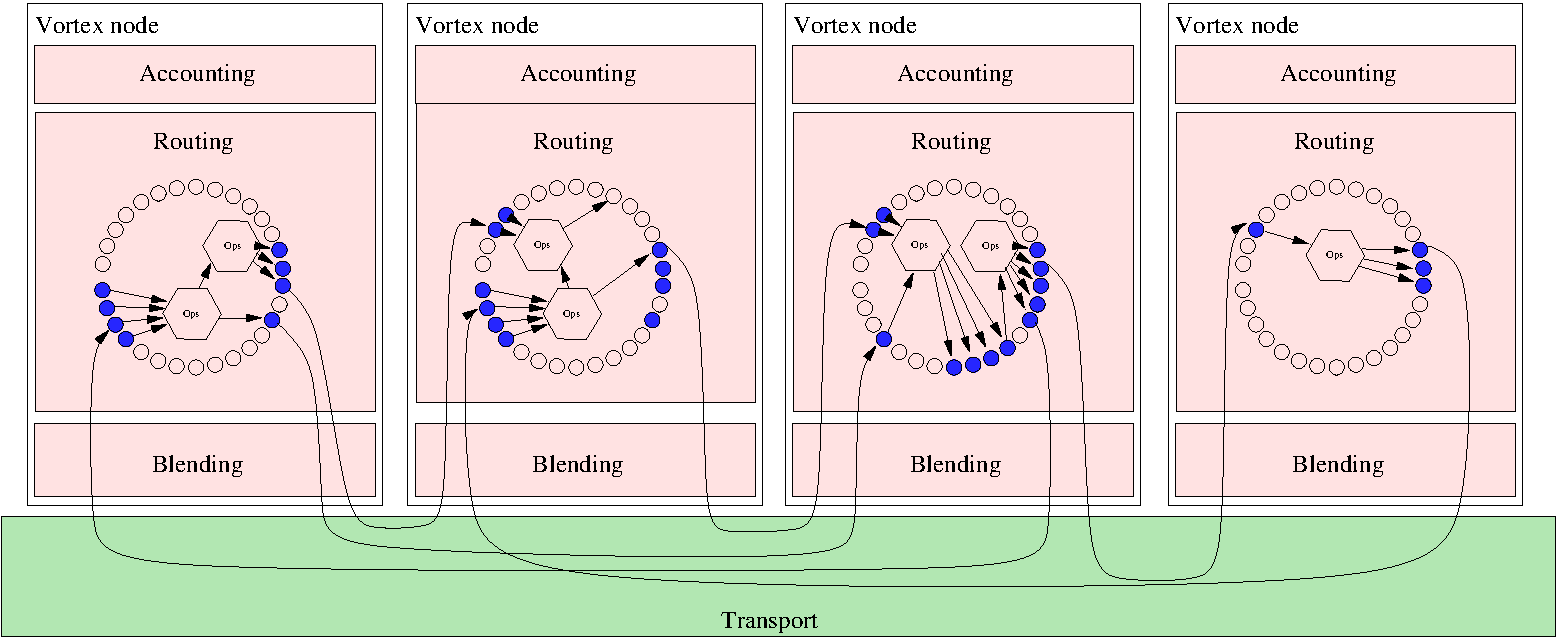
\includegraphics[width=\columnwidth]{inc/roughProtocolDesign.pdf}
	\caption{A generic overview for the protocol showing a circular path of a message}
	\label{fig:roughProtocolDesign}
\end{figure}    

The protocol itself should send messages through a well-known transport protocol (``Transport''). We use this protocol for transporting our messages to the next peer. The messages are hidden within regular messages already using that transport layer. In an ideal implementation, any messages sent by our protocol should be indistinguishable from regular messages (by computers and humans). To achieve this particular task, we introduce a ``blending layer''. This layer usually is specific to the underlying transport layer and may vary.

The ``routing layer'' is the layer that receives and sends messages. It parses only the core protocol, and the data processed here is entirely independent of the underlying transport and blending layer.

The ``accounting layer'' disassembles the received messages into its parts. It then recomposes and stores the messages for further routing. To avoid unsolicited bulk messages (\defref{UBM}) being sent over our media, some accounting is involved. 

The messages passed through such a protocol stack are onionised to offer anonymity from evil nodes. Furthermore, a node should be unable to tell whether a message was intended for a specific node or not. In consequence, we have to guarantee that all nodes, including sender and recipient, offer the same functions and are indistinguishable.

To mitigate size based attacks (an onionised packet typically loses data on its way), we introduce operations that may be applied to a valid message as well as to decoy traffic. The operations must increase and decrease the message in size. The operations must not leak which part is decoy or not. Operations not carried out due to missing data might be either intentionally or a malfunction.

The defined message operations are as follows:
\begin{itemize}
	\item Split a message block into two parts of variable size or join them.\\
	This operation may be used to fan out decoy traffic, to cut off decoy data, or to send multiple parts of a message through different routing nodes.
	\item Encrypt or decrypt a block with a given key.      
	\item Add redundancy information to a stream and send it through multiple channels or recover a partially received message according to the redundancy operation.
\end{itemize}

To avoid making this system attractive to \defref{UBM}, we introduce accounting to make mass mailings more expensive. The system works as follows:
\begin{itemize}
	\item Routing nodes may offer their services at a cost. A participating node may pay a fee or solve a crypto-puzzle to pay for these costs.
	\item The following operations may be cost-effective:
	\begin{itemize}
		\item Getting an ephemeral identity (\defref{eID}) on a node (prerequisite for accounting; See section \ref{sec:ephemeralIdentity}).
		\item Assign a maximum number of messages and bytes in a specified interval to an eID on a node.
		\item Offer information about the known routing network by the node.
		\item Offer information about the current quota of an eID.
	\end{itemize}
\end{itemize}
As we want to keep resource consumption for accounting as low as possible, all quotas are limited to a time interval. Such time-bound quotas guarantee that quota data of an accounting layer does not grow indefinitely. It is up to the node to decide what time duration is still acceptable.

We minimize the possibility of an overload attack against a node. We achieve this with the following precautions:
\begin{itemize}
	\item The message build process is far more complex than the routing carried out by the nodes.
	\item Messages may be processed in parts to minimize the amount of work. After processing the start of a message, a node may already decide whether it will route the message or not.
	\item The protocol minimizes the use of inefficient operations (e.g., asymmetric encryption).
	\item The server may limit specific operations.
\end{itemize}

\subsection{Ephemeral Identity\label{sec:ephemeralIdentity}}
We use accounting on various levels. While we are dealing with anonymity, accounting has still to be linked to some identity. For this reason, we are introducing a term called ``ephemeral identity'' (\defref{eID}).

\begin{quote}
	An eID is a temporary identity, which is defined by the following attributes:
	\begin{itemize}
		\item It is a identity represented by a public key.
		\item It is only valid for a short, limited time-span.
		\item It is not linkable to another identity of any kind.
	\end{itemize}
\end{quote}
The key to this definition is the last point. It is crucial and, at the same time, hard to achieve. In the protocol, any node may request from another node to accept a new eID with a specified quota and a limited lifespan. The node accepting the identity may link its acceptance to the solving of a proof of work puzzle.

\section{Rough Draft of Messages}
For our protocol, we assume the following outline for a message:
\begin{itemize}
	\item Header block\\ 
	This block contains an eID of the sender on the message processing host. It allows the host to decide whether he is willing to process the rest of the message or not. It is essential to know that the identity block contains a symmetric key for decryption of the main block and a secret repeated in the main block. This secret, shared among blocks, keeps a malicious node from exchanging the main block.
	\item Main block\\
	This block contains all information regarding routing and processing data. It furthermore contains the payload data, which may or may not contain messages.
	\begin{itemize}
		\item Routing Blocks\\
		This block contains routing information for all blocks. It furthermore may contain instruction for processing the data blocks and routing/reply blocks for subsequent processing. Routing blocks are not necessarily related to the payload in the same message. They may pick up payloads from other blocks.
		\item payload Block\\
		These Blocks form the payload data. They might contain a message, parts of a message, or decoy material.
	\end{itemize}      
\end{itemize}

The message is picked up from the transport layer by the blending layer. This layer extracts the contained data and passes it to the routing layer. The routing layer extracts the message by decrypting the ephemeral identity block. The accounting layer is called to authorize further processing for the identity. If approved, the routing layer adds the routing blocks to the identity-specific workspace. As soon as the time specified in the routing block arrises, the routing block is processed by following the operations specified within. New messages are assembled and sent. The accounting layer keeps track of the quota regarding the new constructed messages. 

\chapter{Existing Transport Layer Protocols \label{sec:existingTPP}}
In this chapter, we look at the various transport layer protocols. The primary goal is to identify strong candidates as a transport layer. The main focus lies on the following criteria:
\begin{itemize}
	\item Widely adopted (Ct1)\\
	The more widely adopted and used a protocol is, the harder it is for an adversary to monitor (due to the sheer mass), filter, or block the protocol (censorship resistance).
	\item Reliable (Ct2)\\
	Message transport between peers should be reliable. As messages may arrive anytime from everywhere, we do not have means to synchronize the peer partners on a higher level without investing a considerable effort. To avoid this effort, we do look for inherently reliable protocols.
	\item Symmetrical built (Ct3)\\
	The transport layer should rely on a peer to peer base. All servers implement a generic routing that requires no prior knowledge of all possible targets. This criterion neglects centralized infrastructures. This criterion may be dropped, assuming that the routing layer or a specialized transport overlay is responsible for routing.
\end{itemize}

\section{Roundup for Transport Protocols}
\begin{table}[h]
	\centering\tiny
	\begin{tabular}{|l|l|l|l|}\hline
		\diaghead{\theadfont protocol Criteria}{Protocol}{Criteria} & \thead{Ct1: Widely adopted}     & \thead{Ct2: Reliable} & \thead{Ct3: Symmetrically built}\\\hline
		HTTP     & $\checkmark$            & $\checkmark$        & $\times$\\              
		FTP         & $\checkmark$            & $\checkmark$        & $\times$\\
		TFTP     & $\times$                & $\times$            & $\times$\\
		MQTT     & \textasciitilde        & $\checkmark$        & $\times$\\              
		AMQP     & \textasciitilde        & $\checkmark$        & $\times$\\
		CoAP     & \textasciitilde        & \textasciitilde     & $\times$\\
		WAMP     & $\times$                & $\checkmark$        & \textasciitilde\\
		XMPP     & $\checkmark$            & $\checkmark$        & $\checkmark$\\
		SMTP     & $\checkmark$            & $\checkmark$        & $\checkmark$\\
		SMS\footnotemark[1] &             &                     & \\
		MMS         & $\times$                & $\checkmark$        & $\times$\\\hline
	\end{tabular}    
	\caption{comparison of protocols in terms of the suitability as transport layer}
	\label{tab:protoSuitCrit}
\end{table}

In table \ref{tab:protoSuitCrit} we sum up all previously analyzed protocols. We use ``$\checkmark$'' for a fulfilled criterion, ``\textasciitilde'' for a partially fulfilled criterion, and ``$\times$'' for a not fulfilled criterion. This overview shows in compact form protocols identified as strong candidates for use as a transport layer in terms of an anonymizing protocol. 

This table shows that strong identified candidates are SMTP (being already a message sending protocol on asynchronous base) and XMPP (a real-time chat protocol able to attach files. This protocol features end-to-end encryption and signing furthermore). Both have the advantages that they are widely adopted on the Internet and do additional support content (such as alternatives or attachments).

\footnotetext[1]{omitted due to message size being too small}

If assuming an implemented transport layer overlay on the MessageVortex protocol side, HTTP and FTP are suitable candidates as well.

\chapter{Existing Research and Implementations on the Topic \label{sec:existingRD}}
\section{Anonymity Research}
In this section, we collect protocols research related to anonymity. We did not stick to anonymous message transfer. Instead, we took a broad focus in terms of technology and outlined in each protocol strengths and weaknesses identified, which may be relevant to this research.

\subsection{Definition of Anonymity}
\DeclareFixedFootnote{\omitted}{footnotes omitted in quote}
As the definition for Anonymity we take the definition as specified in \cite{anonTerminology}.

\begin{quote}
	Anonymity of a subject means that the subject is not identifiable within a set of subjects, the anonymity set.\omitted
\end{quote}
and
\begin{quote}
	Anonymity of a subject from an attacker's perspective means that the attacker cannot sufficiently identify the subject within a set of subjects, the anonymity set.\omitted
\end{quote}

We define the anonymity set as the set of all possible subjects within a supposed message. The anonymity of a subject towards an observing third party is a crucial factor as it relates directly to our adversary model.

\subsection{\texorpdfstring{$k$}{k}-Anonymity}
$k$-anonymity is a term introduced in \cite{k-anonymous:ccs2003}. This work claims that entities are not responsible for an action if an observer is unable to match a specific action to less than $k$ entities.

The Document distinguishes between \textit{Sender $k$-anonymity}, where the sending entity can only be narrowed down to a set of $k$ entities and \textit{Receiver $k$-anonymity}. 

The size of $k$ is a crucial factor. One of the criteria is the legal requirements of the jurisdiction. Depending on the jurisdiction, it usually is not possible to prosecute someone if an action is not directly coupled to one person. Another criterion might be the decreasing of $k$ over time. If a Vortex account is used, we have to assume that some vortex identities go out of commission over time. If $k$ is chosen according to a legal requirement, it should be taken into account that $k$ might be decreasing over time.

\subsection{\texorpdfstring{$\ell$}{l}-Diversity}
In \cite{machanavajjhala2007diversity} an extended model of $k$-anonymity is introduced. In this paper, the authors emphasize that it is possible to break a $k$-anonymity set if there is additional information available which may be merged into a data set so that a distinct entity can be filtered from the $k$-anonymity set. In other words, if an anonymity set is to tightly specified, additional background information might be sufficient to identify a specific entity in an anonymity set.

It might be arguable that a $k$-anonymity in which a member is not implicitly $k$-anonymous still is sufficient for $k$-anonymity in its sense. However, the point made in this work is right and is taken into account. Their approach is to introduce an amount of invisible diversity into $k$-anonymous sets, so that common background knowledge is no longer sufficient to isolate a single member.

\subsection{\texorpdfstring{$t$}{t}-Closeness}
While $\ell$-diversity protects the identity of an entity, it does not prevent information gain. A subject which is in a class has the same attributes. This is where $t$-closeness\cite{li2007t} comes into play. $t$-closeness is defined as follows:

\begin{quote}
	An equivalence class is said to have $t$-closeness if the distance between the distribution of a sensitive attribute in this class and the distribution of the attribute in the whole table is no more than a threshold. A table is said to have $t$-closeness if all equivalence classes have $t$-closeness.
\end{quote}

\section{Single Use Reply Blocks and Multi-Use Reply Blocks}
Chaum first introduced the use of reply blocks in \cite{CHAUM1}. A routing block, in general, is a structure allowing to send a message to someone without knowing the targets' real address. Reply blocks may be differentiated into two classes ``Single Use Reply Blocks'' (SURBs)  and ``Multi-Use Reply Blocks'' (MURBs). SURBs may be used once while MURBs may be used a limited number of times. 

Within our research, we discovered that if a routing protocol is reproducible, the traffic of a MURB may be used to identify some of the properties of the message. Depending on the type of attack, the block has to be repeated very often. For this reason, we limited the number of replays to a low number. The concept is that we have, in our case a routing block, which might be used up to $n$ times ($0<n<127$). It is easily representable in a byte integer (signed or unsigned) on any system. It is big enough to support human communication sensibly and is big enough to add not too much overhead when rerequesting more MURBs. The number should not be too big because if a MURB is reused, the same pattern of traffic is generated, thus making the system susceptible to statistical attacks.

\section{Censorship}
As a definition for censorship we take
\begin{quote}
	Censorship: the cyclical suppression, banning, expurgation, or editing by an individual, institution, group or government that enforce or influence its decision against members of the public -- of any written or pictorial materials which that individual, institution, group or government deems obscene and ``utterly without redeeming social value,'' as determined by ``contemporary community standards.''
\end{quote}

The definition is attributed to Chuck Stone Professor at the School of Journalism and Mass Communication, University of North Carolina. Please note that ``Self Censorship'' (not expressing something in fear of consequences) is a form of censorship too.

In our more technical we reduce the definition to
\begin{quote}
	Censorship: A systematic suppression, modification, or banning of data in a network by either removal, or modification of the data, or systematic influencing of entities involved in the processing (e.g., by creating, routing, storing, or reading) of this data.
\end{quote}
This simplified definition narrows down the location to the Internet as it is the only relevant location for us.  Furthermore, it limits the definition to the maximum reach within that system.

\subsection{Censorship Resistant}
A censorship-resistant system is a system that allows the entities of the system and the data itself to be unaffected from censorship. Please note that this does not deny the presence of censorship per se. It still exists outside the system. However, it has some consequences for the system itself.

\begin{itemize}
	\item The system must be either undetectable or out of reach for an entity censoring.\\
	The possibility of identifying a protocol or data allows a censoring entity to suppress the use of the protocol itself. 
	\item The entities involved in a system must be untraceable.\\
	Traceable entities would result in a mean of suppressing real-world entities participating in the system.
\end{itemize}

\subsection{Parrot Circumvention}
In \cite{oakland2013-parrot} \citeauthor{oakland2013-parrot} express that it is easy for a human to determine decoy traffic as the content is easily identifiable as generated content. While this is true, there is a possibility here to generate ``human-like'' data traffic to a certain extent. As an adversary may not assume that his messages are replied to, the problem does not boil down to a true Turing test. It remains on a ``passive observer Turing test'', enabling the potential nodes to choose their messages. 

In our design, this is the job covered by the blending layer. The blending layer generates these messages. These messages are context-less or remain in the context of previous conversations.

\subsection{Censorship Circumvention}
Several technical ways have been explored to circumvent censorship. All seem to boil down to the following main ideas:
\begin{itemize}
	\item Hide data
	\item Copy or distribute data to a vast amount of places to improve the lifespan of data
	\item Outcurve censorship measurements
\end{itemize}

In the following section, we look at technologies and ideas dealing with these circumvention technologies.

\subsubsection{Covert Channel and Channel Exploitations}
The original term of covert channels was defined by \citeauthor{Lampson73anote}\cite{Lampson73anote} as 

\begin{quote}
	not intended for information transfer at all, such as the service program's effect on system load.
\end{quote}

This was defined  in such a way to distinguish the message flow from 

\begin{quote}
	legitimate channels used by the confined service, such as the bill.
\end{quote}

The use of a legitimate channel such as SMTP and hide information within this specific channel is not a usage of a covert channel. We refer to this as channel exploitation.

\subsubsection{Steganography}

Steganography is an important part when it comes to unlinking information. In \cite{6828087} and \cite{subhedar2014current} we get a very rough overview. As some of the types and algorithms address specific topics of steganography (e.g., some hide from automatic detection and others address a human message stream auditor), we need to choose carefully. In our specific case, the main idea is to hide within the sheer mass of Internet traffic. As a human auditor screening all the messages is a minor thread, we focus on machine-based censorship. Most of the images sent in SMTP are jpg images (see table \ref{tab:emailAttachments} on page \pageref{tab:emailAttachments}). We limited our search to algorithms capable of hiding binary data within these files. The number of academically researched options was surprisingly low.

After reviewing the options, we decided to go for F5\cite{f5}. It is a reasonably well-researched algorithm which attracted many researchers. The original F5 implementation had a detectable issue with artifacts\cite{F5broken} caused by the recompression of the image. This issue was caused only due to an issue in the reference implementation, and the researchers have provided a corrected reference implementation without the weakness.

% We use https://github.com/matthewgao/F5-steganography

YASS, as described in \cite{solanki2007yass}, was not considered a candidate. Although less researched, researchers found multiple weakness\-es\cite{kodovsky2010modern,li2009steganalysis}.

\subsubsection{Timing Channels}

Timing channels are a specialized form of covert channels. In timing channels, the information itself hides not within the data of the channel, but the usage of the channel is in such a way that it is capable of reflecting the data. As we do not have control over the timing of the transport channel, this is not an option for us.

\section{Cryptography}

Whenever dealing with obfuscating data and maintaining the integrity of data, cryptography is the first tool in the hand of an implementer. A vast amount of research in this area does already exist. For this work, we focussed on algorithms either very well researched and implemented or research, which seem very valuable when putting this work into place. 

In symmetric encryption in this paper always assumes that
\begin{eqnarray}
D^{K_a}\left(E^{K_a}\left(\mathbf{M}\right)\right) & = & \mathbf{M}
\end{eqnarray} 

For a key $K_b\neq K_a$ this means

\begin{eqnarray}
D^{K_a}\left(E^{K_b}\left(\mathbf{M}\right)\right) & \neq & \mathbf{M}\\
D^{K_b}\left(E^{K_a}\left(\mathbf{M}\right)\right) & \neq & \mathbf{M}
\end{eqnarray} 

The following candidates have been analyzed:
\begin{itemize}
	\item AES\\
	NIST announced AES in \citeyear{standard2001announcing} as a result of a contest. The algorithm works with four operations (subBytes, ShiftRows, mixColumns, and addRoundKey). These operations are repeated depending on the key length 10 to 14 times. 
	
	AES is up until now (2018) unbroken. It has been weakened in the analysis described in \cite{tao2015improving}, which reduces the complexity by roughly one to two bits. 
	
	\item Camellia\\
	The camellia algorithm is described in \cite{RFC3713}. The key sizes are 128, 192, and 256. Camellia is a Feinstel cipher with 18 to 24 rounds depending on the key size. Up until today, no publication claims break this cipher. 
\end{itemize}

For all asymmetric encryption algorithm in this paper, we may assume that\ldots

\begin{eqnarray}
D^{K^{-1}_a}\left(E^{K^{1}_a}\left(\mathbf{M}\right)\right) & = & \mathbf{M}\\
D^{K^{1}_a}\left(E^{K^{-1}_a}\left(\mathbf{M}\right)\right) & = & \mathbf{M}
\end{eqnarray} 

It is important that 
\begin{eqnarray}
D^{K^{-1}_a}\left(E^{K^{-1}_a}\left(\mathbf{M}\right)\right) & \neq & \mathbf{M}\\
D^{K^{1}_a}\left(E^{K^{1}_a}\left(\mathbf{M}\right)\right)   & \neq & \mathbf{M}
\end{eqnarray} 

And for any other Keypair $K^{p}_a \neq K^{p}_b$
\begin{eqnarray}
D^{K^{-1}_b}\left(E^{K^{1}_a}\left(\mathbf{M}\right)\right)  & \neq & \mathbf{M}\\
D^{K^{1}_b}\left(E^{K^{1}_a}\left(\mathbf{M}\right)\right)   & \neq & \mathbf{M}\\
D^{K^{-1}_b}\left(E^{K^{-1}_a}\left(\mathbf{M}\right)\right) & \neq & \mathbf{M}\\
D^{K^{1}_b}\left(E^{K^{-1}_a}\left(\mathbf{M}\right)\right)  & \neq & \mathbf{M}
\end{eqnarray} 

The number of crypto algorithms was higher than the steganography options. When looking for well-researched algorithms basing on different mathematical problems and having well-defined outlines, numbers dropped dramatically again.

\begin{itemize}
	\item RSA\\
	In \citeyear{Rivest:1978:MOD:359340.359342} the authors \citeauthor{Rivest:1978:MOD:359340.359342} published with \cite{Rivest:1978:MOD:359340.359342} a paper which did revolutionize cryptography for years. In their paper, the authors described an encryption method later to be called RSA, which required a key pair ($K_a$) referenced as public ($K^{1}_a$) and private keys ($K^{-1}_a$). The novelty of this system was that anything encrypted with the public key was only decryptable with the private key and vice versa.
	
	RSA is up until the day of writing this paper not publicly know to be broken (unless a too small key size is used). However -- \citeauthor{Shor97polynomial-timealgorithms} described in \citeyear{Shor97polynomial-timealgorithms} an algorithm which should enable quantum computers to break RSA far faster than done with traditional computers. In the section \ref{sec:keySize} we do elaborate these effects further.
	\item ECC\\
	The elliptic curves were independently suggested by \cite{Miller1986} and \cite{Koblitz04guideto} in 1986. Elliptic curve Cryptography started to be widely deployed in the public space in 2006. Since then, it seems to compete very well with the well established RSA algorithm. While being similarly well researched ECC, has the advantage of far shorter key sizes for the same grade of security.
	\item McElliece\\
	McEliece was first implemented and then removed again. The key size to gain equivalent security to RSA1024 was $\approx 1MB$. This was impractical and thus discarded again. This was done, although there is up until now no known quantum capable algorithm reducing the key size of McEliece.
	\item NTRU\\
	In \cite{Hoffstein1998} \citeauthor{Hoffstein1998} described the NTRU algorithm. The inclusion of this algorithm was disputed as it is patented in the united states as US7031468. It was included because the company Security Innovation holding the patent, released the NTRU algorithm on March \thanks{28} 2018 into the public domain according to a blog entry on the company website. While NTRU is not as well researched as RSA, it has been around for more than 20 years without being significantly affected by known attacks.
	\item ElGammal\\
	We rejected ElGamal as a cryptosystem to include. It bases on the same mathematical problems for cryptoanalysis as RSA (discreet logarithms) but is not as common as RSA.
\end{itemize}


\subsection{Homomorphic encryption}
Homomorphic encryption, as introduced in \cite{feldman1987practical}, was from the beginning a strong candidate to be used within our work. Unfortunately, we did not find a way to apply the core addRedundancy operation in homomorphic encryption. Transforming the original data to the GF space in an efficient way to apply matrices was not doable and thus rejected.

%\cite{Gentry:2009:FHE:1536414.1536440} %FIXME dangling reference

\subsection{Deniable Encryption and Deniable Steganography}

Deniable encryption and deniable steganography have been considered out-of-bounds for this work. The main reason is that the presence of encryption (which is not deniable in both cases) may be sufficient for a censor to block a message. Adding a layer to make sure that encryption or steganography is deniable, does not add valuable properties to our system as the sheer presence of encryption might be sufficient for censorship. 

\subsection{Key Sizes\label{sec:keySize}}

The question of key sizes is hard to answer as it depends on the current and future possibilities of an adversary, which is again depending on not foreseeable research. We tried to collect a couple of recommendations.

\href{http://www.ecrypt.eu.org/}{Encrypt II (http://www.ecrypt.eu.org/)} recommends currently for a ``foreseeable future'' 256 Bits for symmetric encryption and for asymmetric encryption based on factoring modulus 15424 Bits. Elliptic Curve Cryptography and Hashing should be sufficient if used with at least 512 Bits. If the focus is reduced to the next $\approx$ 20 years, then the key size recommendations are reduced to 128 Bit for symmetric encryption, 3248 Bits for factoring modulus operations, and 256 Bits for elliptic curves and hashing.

According to the equations proposed by \citeauthor{Lenstra04keylength.} in \cite{Lenstra04keylength.} an asymmetric key size of 2644 Bits respectively symmetric key length of 95 Bits, or 190 Bits for elliptic curves and hashing should be sufficient for security up to the year 2048. 

According to \cite{CNSASuite} (superseding well known and often used \cite{nsa-fact-sheet-B}) data classified up to ``top secret'' should be signed with RSA 3072+ or ECDSA P-384.  For symmetric encryption, they recommend AES 256 Bits, for Hashing at least SHA-384 and for Elliptic curves a 384 Bit sized key.

As it might seem not a wise idea to consider the recommendation of a potential state-sponsored adversary and the Formulas proposed by \citeauthor{Lenstra04keylength.} do not explicitly take quantum computers into account we follow the recommendations of ENCRYPT II.

Furthermore, taking all recommendations together, it seems that all involved parties assume the most trust in elliptic curves rather than asymmetric encryption based on factoring modulus.

\subsection{Cipher Mode}
The cipher mode defines how multiple blocks encrypted with the same key are handled. Main characteristics of cipher modes to us are:
\begin{itemize}
	\item Parallelisable\\ 
	Can multiple parts of a plaintext be encrypted simultaneously? This feature is important for multi CPU and multi-core systems as they can handle parallelizable more efficiently by distributing them on multiple CPUs.
	\item Random access in decryption\\
	Random access on decryption allows efficient partial encryption of a ciphertext.
	\item Initialisation vector\\
	An initialization vector has downsides and advantages. On the downsides is the fact that an initialization vector must be shared with the message or before distributing it. It is essential to understand that the initialization vector itself usually is not treated as a secret. It is not part of the key.
	\item Authentication\\
	Authentication guarantees that the deciphered plaintext has been unmodified since encryption. It does not make a statement over the identity of the party encrypting the text. Such an identifying authentication is referred to as signcryption.
\end{itemize}

We evaluated the most common cipher modes for suitability. For MessageVortex, we focussed on modes that have the properties parallelizable, random access, and do not do authentication. The main focus, besides the characteristics mentioned above, was on the question of whether there is an open implementation available in java, which is reasonably tested.

\begin{itemize}
	\item ECB (Electronic Code Book)\\
	ECB is the most basic mode. Each block of the cleartext is encrypted on its own. This results in a big flaw: blocks containing the same data will always transform to the same ciphertext. This property makes it possible to see some structures of the plain text when looking at the ciphertext. This solution allows the parallelization of encryption, decryption, and random access while decrypting. Due to these flaws, we rejected this mode.
	\item CBC (Cypher Block Chaining)\\  
	CBC extends the encryption by xor'ing an initialization vector into the first block before encrypting. For all subsequent blocks, the ciphertext result of the preceding block is taken as xor input. This solution does not allow parallelization of encryption, but decryption may be paralleled, and random access is possible. As another downside, CBC requires a shared initialization vector. As with most IV bound modes, an IV/key pair should not be used twice, which has implications for our protocol.
	\item PCBC (Propagation Cypher Block Chaining)\\
	CBC extends the encryption by xor'ing, not the ciphertext but a xor result of ciphertext and plaintext. This modification denies parallel decryption and random access compared to CBC.
	\item EAX\\      
	EAX has been broken in 2012\cite{minematsu2013attacks} and is therefore rejected for our use.
	\item CFB (Cypher Feedback)
	CFB is specified in \cite{dworkin2001recommendation} and works precisely as CBC with the difference that the plain text is xor'ed and the initialization vector, or the preceding cipher result is encrypted. CFB does not support parallel encryption as the ciphertext input from the preceding operation is required for an encryption round. CFB does, however, allow parallel decryption and random access.
	\item OFB\\
	\cite{dworkin2001recommendation} specifies OFB and works exactly as CFB except for the fact that not the ciphertext result is taken as feedback but the result of the encryption before xor'ing the plain text. This denies parallel encryption and decryption, as well as random access.
	\item OCB (Offset Codebook Mode)\\
	This mode was first proposed in \cite{rogaway2003ocb} and later specified in \cite{krovetz-ocb-04}. OCB is specifically designed for AES128, AES192, and AES256. It supports authentication tag lengths of 128, 96, or 64 bits for each specified encryption algorithm. OCB hashes the plaintext of a message with a specialized function $H_{OCB}(\mathbf{M})$. OCB is fully parallelizable due to its internal structure. All blocks except the first and the last can be encrypted or decrypted in parallel.
	\item CTR\\
	CTR is specified in \cite{lipmaa2000ctr} and is a mixture between OFB and CBC. A nonce concatenated with a counter incrementing on every block is encrypted and then xor'ed with the plain text. This mode allows parallel decryption and encryption, as well as random access. Reusing IV/Key-pairs using CTR is a problem as we might derive the xor'ed product of two messages. This problem only applies where messages are not uniformly random such as in an already encrypted block.
	\item CCM\\
	Counter with CBC-MAC (CCM) is specified in \cite{RFC3610}. It allows to pad and authenticate encrypted and unencrypted data. It furthermore requires a nonce for its operation. The size of the nonce is dependent on the number of octets in the length field. In the first 16 bytes of the message, the nonce and the message size is stored. For the encryption itself, CTR is used. It shares the same properties as CTR. 
	
	It allows parallel decryption and encryption as well as random access.
	\item GCM (Galois Counter Mode)\\
	GCM has been defined in \cite{mcgrew2004galois}, and is related to CTR but has some major differences. The nonce is not used (just the counter starting with value 1). To authenticate the encryption, an authentication token $auth$ is hashed with $H_{GFmult}$ and then xor'ed with the first cipher block. All subsequent cipher blocks are xor'ed with the previous result and then hashed again with $H_{GFmult}$. After the last block the output $o$ is processed  as follows: $H_{GFmult}(o\bigoplus (len(A)||len(B))) \bigoplus E^{K^0}(counter_0)$. As a result, GCM is not parallelizable and does not support random access.
	
	The mode has been analyzed security-wise in \citeyear{mcgrew2004security} and showed no weaknesses in the analyzed fields \cite{mcgrew2004security}. 
	
	GCM supports parallel Encryption and decryption. Random access is possible. However, authentication of encryption is not parallelizable. The authentication makes it unsuitable for our purposes. Alternatively, we could use a fixed authentication string.
	\item XTS (XEX-based tweaked-codebook mode with ciphertext stealing)\\
	This mode is standardized in IEE 1619-2007 (soon to be superseded). A rough overview of XTS may be found at \cite{Martin2010}. It was developed initially for Disks offering random access and authentication at the same time. 
	\item CMC (CBC-mask-CBC) and EME (ECB-mask-ECB)\\ 
	In \cite{Halevi:2003} \citeauthor{Halevi:2003} introduces a cipher mode which is extremely costly as it requires two encryptions. CMC is not parallelizable due to the underlying CBC mode, but EME is. 
	\item LRW\\
	LRW is a tweakable narrow-block cipher mode described in \cite{tschorsch:translayeranon}. This mode shares the same properties as EBC but without the weakness of the same clear text block resulting in the same ciphertext. Similarly to XEX, it requires a tweak instead of an IV.
\end{itemize}

\subsubsection{Summary of Cipher Modes}

\begin{table}[ht]
	\centering\tiny
	\begin{tabular}{|l|l|l|l|l|}\hline
		\diaghead{\theadfont Mode Criteria}{Mode}{Criteria}         & \thead{auth}  &\thead{Requires IV}               & \thead{parallelisable}     & \thead{random access}\\
		\hline
		CBC                                                            & $\times$        & $\checkmark$                      & $\times$                & $\times$\\                      
		CCM                                                            & $\times$        & $\checkmark$                      & $\times$                   & $\times$\\
		CFB                                                            & $\times$        & $\checkmark$                      & $\checkmark$            & $\checkmark$\\              
		CTR                                                            & $\times$        & $\checkmark$                      & $\checkmark$               & $\checkmark$\\              
		ECB                                                            & $\times$        & $\times$                          & $\checkmark$            & $\checkmark$\\   
		GCM                                                            & $\checkmark$    & $\checkmark$                      & $\times$                   & $\times$\\              
		OCB                                                            & $\checkmark$    & $\times^{\text{includes auth}}$ & $\times$                 & $\times$\\              
		OFB                                                            & $\times$        & $\checkmark$                      & $\times$                & $\times$\\              
		PCBC                                                        & $\times$        & $\checkmark$                      & $\times$                & $\times$\\              
		XTS                                                            & $\times$        & $\checkmark$\footnote{Requires tweak instead of IV}& $\checkmark$                & $\times$\\
		LRW                                                            & $\times$        & $\checkmark$\footnote{Requires tweak instead of IV}& $\checkmark$                & $\checkmark$\\              
		CMC                                                         & $\times$        & $\checkmark$\footnote{Requires tweak instead of IV}& $\times$                    & $\times$\\           
		EME                                                         & $\times$        & $\checkmark$\footnote{Requires tweak instead of IV}& $\checkmark$                    & $\checkmark$\\              
		\hline          
	\end{tabular}    
	\caption{comparison of encryption modes in terms of the suitability}
	\label{tab:ModeSuitCrit}
\end{table}

\subsection{Padding}
A plain text stream may have any length. Since we always encrypt in blocks of a fixed size, we need a mechanism to indicate how many bytes of the last encrypted block may be safely discarded. 

Different paddings are used at the end of a cipher stream to indicate how many bytes belong to the decrypted stream.

\subsubsection{RSAES-PKCS1-v1\_5 and RSAES-OAEP}
This padding is the older of the paddings standardized for PKCS1. It is basically a prefix of two bytes followed by a padding set of non zero bytes and then terminated by a zero byte and then followed by the message. This patting may give a clue if decryption was successful or not. RSAES-OAEP ist the newer of the two padding standards 

\subsubsection{PKCS7} 
This padding is the standard used in many places when applying symmetric encryption up to 256 bits key length. The free bytes in the last cipher block indicate the number of bytes being used. This makes this padding very compact. It requires only 1 Byte of functional data at the end of the block. All other bytes are defined but not needed.

\subsubsection{OAEP with SHA and MGF1 padding} 
This padding is closely related to RSAES-OAEP padding. The hash size is, however, bigger, and thus, the required space for padding is much higher. OAEP with SHA and MGF1 Padding is used in asymmetric encryption only. Due to its size, it is important to note that the payload in the last block shrinks to $keySizeInBits/8-2-MacSize/4$.

In our approach, we have chosen to allow these four paddings. The allowed sha sizes match the allowed hash sizes chosen above. It is important to note that padding costs space at the end of a stream. Since we are always using one block for signing, we have to take care that the chosen signing mac plus the bytes required for padding do not exceed the key size of the asymmetric encryption. While this usually is not a problem for RSA as there are keys 1024+ Bits required, it is an important problem for ECC algorithms as there are much shorter keys required to achieve an equivalent strength compared to RSA. 

We have introduced an additional type of padding not related to these paddings. We required for the addRedundancy the following unique properties. Unfortunately, we were unable to find any padding which matched the following properties simultaneously:

\begin{itemize}
	\item Padding must not leak successful decryption\\
	For our addRedundancy operation, we required padding that had no detectable structure as a node should not be able to tell whether a removeRedundancy operation did generate content or decoy. 
	\item Padding of more than one block\\
	Due to the nature of the operation, it is required to be able to pad more than just one block.
\end{itemize}

Details of this padding are described in the section "Add and Remove Redundancy Operations'' in \ref{app:rfcMessageVortexMain}. 

\section{Routing}

If we can follow data from a source to a destination, we may safely assume that the participants of this data exchange are no longer anonymous. So special care should be taken to this aspect. In the past, several approaches have been made to avoid the detection of data while routing. In the following sections, we will look at some basic concepts which have been proposed up until today. We describe their concept and have a look at their weaknesses discovered so far.

In \nameref{sec:sysImpl}, we analyze some related real-world systems regarding how they work and how they have been attacked in the past.

\subsection{Mixing\label{sec:mixnets}}
Mixes have been first introduced by \citetitle{CHAUM1}\cite{CHAUM1} in \citeyear{CHAUM1}. The basic concept in a mix goes as follows. We do not send a message directly from the source to the target. Instead, we use a kind of proxy server or router in between which picks up the packet, anonymizes it, and forwards it either to the recipient or another mix. If we assume that we have at least three mixes cascaded, we then can conclude that:
\begin{itemize}
	\item Only the first mix knows the true sender
	\item All intermediate mixes know neither the true sender nor the true recipient (as the data comes from mixes and is forwarded to other mixes) 
	\item Only the last mix knows the final recipient.
\end{itemize}

This approach (in this simple form) has several downsides and weaknesses.

\begin{itemize}
	\item In a low latency network, the message may be traced by analyzing the timing of a message.
	\item We can emphasize a path by replaying the same message multiple times (assuming we control an evil node), thus discovering at least the final recipient.
	\item If we can ``tag'' a message (with content or attribute), we then may be able to follow the message.
\end{itemize}

In \citeyear{RP03-1} \citeauthor{RP03-1} analyzed the suitability for mixes as an anonymizing network for masses. They concluded that there are three possibilities to run mixes.
\begin{itemize}
	\item Commercial, static MixNetworks
	\item Static MixNetworks operated by volunteers
	\item Dynamic MixNetworks
\end{itemize}
They concluded that in an ideal implementation, a dynamic mix network where every user is operating a mix is the most promising solution as static mixes always might be hunted by an adversary.

\subsection{Onion Routing}
Onion routing is a further development of the concept of mixes. In onion routers, every mix gets a message which is asymmetrically encrypted. By decrypting the message, he gets the name of the next-hop and the content which he has to forward. The main difference in this approach is that in traditional mix cascades, the mix decides about the next hop. In an onionised routing system, the message decides about the route it is taking. 

While tagging attacks are far harder (if we exclude side-channel attacks to break sender anonymity), the traditional attacks on mixes are still possible. So when an adversary is operating entry and exit nodes, it is straightforward for them to match the respective traffic.

One very well known onion routing network is Tor (\href{https://www.torproject.org}{https://www.torproject.org}). For more information about tor see section \ref{sec:tor}.

\subsection{Crowds}

Crowds is a network that offers anonymity within a local group. It works as follows:

\begin{itemize}
	\item All users add themselves to a group by registering on a so-called ``blender''.
	\item All users start a service (called JonDo).
	\item Every JonDo takes any received message (might be from him as well) and sends it with a 50\% chance either to the correct recipient or to a randomly chosen destination
\end{itemize}

While crowds as specified in \cite{crowds:tissec} does anonymize the sender from the recipient rather well, the system offers no protection from someone capable of monitoring crowds traffic. The system may, however, be easily attacked from within by introducing collaborating johndos. It has been further developed to D-Crowds \cite{DBLP:conf/esorics/DanezisDKT09}, ADU/RADU \cite{Munoz-Gea2008}, Freenet\cite{freenet} and many others. 

\subsection{Mimic routes}
Mimics are a set of statical mixes which maintain a constant message flow between the static routes. If legitimate traffic arrives, the pseudo traffic is replaced by legitimate traffic. An outstanding observer is thus incapable of telling the difference between real traffic and dummy traffic.

If centralized mixes are used, the system lacks the same vulnerabilities of sizing and observing the exit nodes as all previously mentioned systems. If we assume that the sender and receiver operate a mixer by themselves, the system would be no longer susceptible to timing or sizing analyses. The mimic routes put a constant load onto the network. This bandwidth is lost and may not be reclaimed. It does not scale well as every new participant increases the need for mimic routes and creates (in the case of user mixes) a new mimic load.

\subsubsection{DC Networks}
DC networks are based on the work \citetitle{chaum-dc} by \citeauthor{chaum-dc}\cite{chaum-dc}. In this work, \citeauthor{chaum-dc} describes a system allowing a one-bit transfer (The specific paper talks about the payment of a meal). Although all participants of the DC net are known, the system makes it unable to determine who has been sending a message. The message in a DC-Net is readable for anyone. This network has the downside that a cheating player may disrupt communication without being traceable.

Several attempts have been made to strengthen the proposal of Chaum\cite{golle:eurocrypt2004}\cite{disco}. However, no one succeeded without introducing significant downsides on the privacy side.
\subsubsection{Annonymous Remailer\label{sec:remailer}}
Remailers have been in use for quite some time. There are several classes of remailers, and all of them are somehow related to Mixnets. There are ``types'' of remailers defined. Although these ``types'' offer some hierarchy, none of the more advanced ``types'' seem to have more than one implementation in the wild. 

Pseudonymous Remailers (also called Nym Servers) take a message and replace all information pointing to the original sender with a pseudonym. This pseudonym may be used as an answer address. The most well known pseudonymous remailer possibly was anon.penet.fi run by Johan Helsingius. This service has been forced several times to reveal a pseudonyms true identity before Johan Heösingius decided to shut it down. For a more in-depth discussion of Pseudonymous Remailers see \ref{sec:remPseudo}

Cypherpunk remailers forward messages like pseudonymous remailers. Unlike pseudonymous remailers, Cypherpunk remailers decrypt a received message, and its content is forwarded without adding a pseudonym. A reply to such a message is not possible. They may, therefore, be regarded as an ``decrypting reflector'' or a ``decrypting mix'' and may be used to build an onion routing network for messages. For a more in-depth discussion of Type-I-Remailers, see \ref{sec:remCypherpunk}.

Mixmaster remailers are very similar to Cypherpunk remailers. Unlike them, Mixmaster remailers hide the messages, not in an own protocol, but use SMTP instead. While using SMTP as a transport layer, Cypherpunk remailers are custom (non-traditional mail) servers listening on port 25. For a more in-depth discussion of type-II-remailers, see \ref{sec:remMixmaster}.

Mixminion remailers extend the model of Mixmaster remailers. They still use SMTP but introduce new concepts. New concepts in Mixminion remailers are:
\begin{itemize}
	\item Single Use Reply Blocks (SURBs)
	\item Replay prevention
	\item Key rotation
	\item Exit poicies
	\item Dummy traffic
\end{itemize}
For a more in depth discussion of Mixminion remailers see \ref{sec:remMixminion}.

\section{System Implementations\label{sec:sysImpl}}
The following sections emphasize on implementations of anonymizing (and related) protocols regardless of their usage in the domain of messaging and anonymity. It is a list of system classes or their specific implementations together with a short analysis of strengths and weaknesses. 

Wherever possible, we try to refer to sources. If systems are no longer in use or have never been adopted outside the scientific community, we try to refer to publicly available sources. Some of them do not even have a rudimentary implementation. Instead, they are limited to an idea or a simulator.

If a system shows strong similarities in parts, then we emphasize on these parts and analyze the findings and attacks.

\subsection{Pseudonymous Remailer\label{sec:remPseudo}}
The basic idea of remailers was discussed in \cite{CHAUM1}. The most well-known remailer was probably anon.penet.fi, which operated from 1993 to 1996. This type of remailer is often referred to as type-0-remailer.

In principle, an anonymous remailer works as an ordinary forwarding SMTP server. The only difference is that it strips off all header fields except for ``from'', ``to'', and ``subject'' and then replaces the sender and recipient address with pseudonyms (if any). 

As the example shows, this kind of remailer is easily attackable by an authority. Since the remailer knows tuples of pseudonyms and their respective real identities, it may be forced to reveal true identities. Furthermore, the message may be monitored at the server or on its way, and then due to the unmodified content matching is easy.

This remailer offers, therefore, no protection against an adversary defined in our problem.

\subsection{Babel}
Babel was an academic system defined in a paper by \citeauthor{babel} in \citeyear{babel}\cite{babel}. It has been developed at IBM Zurich Research Laboratory. It was a mixing system using onionized addresses. The sender remains anonymous while he may provide a reply routing block called RPI. If both parties would like to remain anonymous, the RPI of the initiator is deployed in a forum thread. Anyone using this block adds an RPI for its address to the message.

This system has all the disadvantages of a system using MURBs. Traffic highlighting and similar attacks are possible.

\subsection{Cypherpunk-Remailer\label{sec:remCypherpunk}}
With the failing of anon.penet.fi, it became clear that the weakest spot of a single server infrastructure the information stored on the server and the vulnerability of their owner. The new type-1 remailers score over the existing type-1 remailers by using encryption for the message. By combining multiple type-1 remailers, an onion-like structure of the message was achievable. 

This approach was promising, but it was still observable. An observation was possible in the example of correlating the message sizes and timing information.

\subsection{Mixmaster-Remailer\label{sec:remMixmaster}}
Like Cypherpunk remailers, the Mixmaster remailers were working with onion-like encrypted messages. In contrast to type-1 remailers, the use of cascading mixes became systematic.

\subsection{Mixminion-Remailer\label{sec:remMixminion}}
Mixminion was the standard implementation of a type-3 remailer. It tried to address many issues previously not solved. A Mixminion router splits messages in equally sized chunks and supports SURBs. Furthermore,  replay protection and key rotation were available. Unlike the previous remailer types, Mixminion was no longer using SMTP as the transport protocol. Instead, Mixminion introduced a new transport protocol. The sources of this remailer are available on GitHub under https://github.com/mixminion/mixminion.

\subsection{Tarzan}
Tarzan is a P2P IP protocol using UDP to communicate. It is specified in \cite{tarzan:ccs02}. Tarzan nodes may be used to anonymize Internet traffic in general. An initiator on the original sender machines encapsulates traffic into a layered UDP package and sends the package through a mix like relayd's. The last relayd acts as an exit node. A replier may send answers the opposite way. Each relayd knows its next and previous relayd. To minimize the impact of observation, Tarzan forwards packets only every 20ms and features replay protection.

\subsection{AN.ON}
AN.ON, as suggested in \cite{federrath2003system}, is a mixing network. It generates messages in equally sized chunks and sends them in fixed time slots after random mixing. Its implementation is called JAP and may be found under https://anon.inf.tu-dresden.de/. JAP is many ways similar to the capabilities of ToR. The network was at the time of writing a lot smaller (10 JonDos compared to 6500 relays in the ToR network).

\subsection{MorphMix}
MorphMix is another mix network. It is specified in \cite{morphmix:wpes2002}. It was a circuit-based mix system for networking anonymity. The core of the network was collision detection. This detection has been circumvented by \cite{morphmix:pet2006}. Since then, no new papers have been published, and the project seems to be dead.

\subsection{SOR (SSH-based onion routing)}
SOR \cite{Egners_2012} is blaming the complex and monocultural landscape of anonymizing software and proclaims a simple approach based on onionized SSH tunnels. While the approach is both simple and effective, it is not suitable against a powerful adversary. First, he may be able to snoop the forwarding when on the system. Second, due to the timing behavior, tunnels belonging to each other may be identified, and third, the package size information does leak as well.

\subsection{SCION}
SCION\cite{perrig2017scion} is a clean slate Internet protocol. While SCION is not really an anonymizing protocol it contains many interesting features. Unlike with the traditional networks, we have the possibility of influencing the routing of data within SCION. Furthermore, with PHI\cite{chen2017phi} and Dovetail\cite{sankey2014dovetail} they could feature strong and fast anonymity features. Unfortunately, as this is a clean slate Internet design, it is not available commonly and as it is easy identifiable it enables censorship again. First, the protocol is easily identifiable and can be censored.

\subsection{Tor\label{sec:tor}}
Tor is one of the most common onion router networks these days and onionizes generic TCP streams. It is specified in \cite{tor-spec}. It might be considered one of the most advanced networks since it has a considerable size, and much research has been done here.

According to \cite{onion-routing:pet2000} ToR is a network consisting of multiple onion routers. Each client first picks an entry node. Then it establishes an identity, gets a listing of relay servers, and chooses a path through multiple onion routers. The temporary identity links to such a path and should be changed on a regular base along with its identity. Transferring data works by splitting the data into equally sized cells of 512 bytes.

There is a centrally organized directory in the tor network, knowing all tor relay servers. Any Tor relay server may be a directory server as well. 

Many attacks involving the Tor networks have been discussed in the academic world such as \cite{hs-attack06,esorics13-cellflood,bauer:wpes2007,esorics12-torscan,oakland2013-trawling,danner-et-al:tissec12,congestion-longpaths} and some have even been exploited actively. In the best case, the people discovering the attacks did propose mitigation to the attack. Some of these mitigations flowed back into the protocol. Some general thoughts of the attacks should be emphasized here for treatment in our protocol.

Being an exit node may be a problem in some jurisdictions. In general, it seems to be accepted that routing traffic with unknown content (to the routing node) is not regarded as illegal per se. So by being unable to tell malicious or illegal traffic apart from legitimate traffic, this is not a problem. However -- being an exit node can mean that unencrypted and illegal traffic is leaving the routing traffic. In this specific case, operators of a relay node might fear legal prosecution. Tor nodes may proclaim themselves as  `` non-exit nodes''  to avoid the possibility of legal prosecution.

Furthermore, several DoS-Attacks have been carried out to overload parts of the Tor network. Most of them do a bandwidth drain on the network layer.

Attacking anonymization has been done in several ways. First of all, the most common attack is a time-wise correlation of packets if in control of an entry and an exit node. A massive attack of this kind was published in 2014 and has been published on the tor website (\href{https://blog.torproject.org/blog/tor-security-advisory-relay-early-traffic-confirmation-attack}{relay early traffic confirmation attack}). This attack was possible because tor is a low latency network. Another attack is to identify routes through tor by statistically analyze the traffic density in the network between nodes. More theoretical attacks focus on the possibility of controlling the directory servers to guarantee that an entity may be deanonymized because it is using compromised routers.

Generally, the effectiveness of the monitoring of single nodes or whole networks is disputed. According to a study by \citeauthor{ccs2013-usersrouted} in \citeyear{ccs2013-usersrouted}\cite{ccs2013-usersrouted}, a system in the scale of PRISM should be able to correlate traffic of 95\% of the users within a ``few days''. Other sources based on the Snowden Papers claim that NSA was unable so far to de-anonymize users of  ToR. However, since these papers referenced to ``manual analysis'', the statement may be disputed when looking at automated attacks as well.

It is, according to \url{https://www.torproject.org/docs/pluggable-transports}, impossible to use transborder ToR traffic in at least China, Uzbekistan, Iran, and Kazakstan. In censored countries, ToR offers so-called bridged Transports. Currently deployed transports in the standard ToR browser bundle package are obfs4, meek, FTE, and ScrambleSuit. Only meek is listed as working in China. Meek achieves this by hiding its traffic in a standard protocol (https).

\cite{saleh2018shedding} is an excellent survey listing recent developments and attacks within the ToR project.

\subsection{\texorpdfstring{$I^2P$}{I2P}}
The name $I^2P$ is a derived from  ``Invisible Internet Project'' according to \href{https://geti2p.net/}{geti2p.net}. The system itself is comparable to ToR for its capabilities. Mayor differences are:
\begin{itemize}
	\item P2P based
	\item Packet-switched routing (tor is ``circuit-switched'')
	\item Different forward and backward routes (called tunnels)
	\item Works pseudonymously
	\item Supports TCP and UDP
\end{itemize}

$I^2P$ has not attracted as much attention as ToR so far. So it is hard to judge upon its real qualities.

In \citeyear{pets2011-i2p} \citeauthor{pets2011-i2p} presented in \cite{pets2011-i2p} an attack. As $I^2P$s security model is chosen based on IP addresses, the authors propose to use several cloud providers in different B-Class networks. By selectively flooding peers, an adversary may extract statistical information. The paper proposes an attack based on the heuristic performance-based peer selection. The main critics of the paper were that the peer selection might be influenced by an adversary enabling him to recover $I^2P$ has not attracted as much attention as ToR so far. So it is hard to judge upon its real qualities.

In \citeyear{pets2011-i2p} \citeauthor{pets2011-i2p} presented in \cite{pets2011-i2p} an attack. As $I^2P$s security model is chosen based on IP addresses, the authors propose to use several cloud providers in different B-Class networks. By selectively flooding peers, an adversary may extract statistical information. The paper proposes an attack based on the heuristic performance-based peer selection. The main critics of the paper were that the peer selection might be influenced by an adversary enabling him to recover data on a statistical base.


\subsection{Freenet}
Freenet was initially designed to be a fully distributed data store\cite{freenet}. Documents are stored in an encrypted form. Downloaders must know a document descriptor called CHK containing the file hash, the key, and some background about the crypto being used. A file is stored more or less redundantly based on the number of accesses to a stored file. The primary goal of Freenet is to decouple authorship from a particular document. It furthermore provides fault-tolerant storage, which improves caching of a document if requested more often.

Precisely as $I^2P$, Freenet is not analyzed thoroughly by the scientific world. 

The Freenet features two protocols FCPv2 acts as the client protocol for participating in the control of the Freenet storage. The Freenet client protocol allows us to insert and retrieve data, to query the network status, and to manage Freenet nodes directly connected to an own node. FCPv2 operates on port 9481, and blocking is thus easy, as it is a dedicated port. 

The Freenet project seems to be under active development as pages about protocols were updated in the near past (Last update on the FCPv2 Page was July \nth{5} 2016 at the time of writing).

\subsection{Herbivore}
Herbivore is a network protocol designed by \citeauthor{herbivore:tr} in \cite{herbivore:tr}. It is based on the dining cryptographers paper\cite{chaum-dc}. At the time of writing, no herbivore client or an actual protocol implementation could be found on the Internet. Wikipedia lists Herbivore as ``dormant or defunct''.

\subsection{Dissent}
Dissent is defined in \cite{Corrigan-Gibbs:2010:DAA:1866307.1866346}. It is an anonymity network based on DC-nets. A set of servers forms these DC-nets. At least one of the servers in the used net must be trustworthy, and none may be misbehaving. A server failure results in the stall of all message delivery using this server.

\subsection{\texorpdfstring{$\mathcal{P}^5$}{P5}}
The Peer-to-Peer Personal Privacy Protocol is defined in \cite{sherwood-protocol}. It provides sender-, receiver- and sender-receiver anonymity. According to the project page of $\mathcal{P}^5$, there is only a simulator available for the protocol.

The transport layer problematic has been wholly ignored. As there is no precise protocol specification but only a rough outline about the messaging and the crypto operations, $\mathcal{P}^5$ offers minimal possibilities for analysis.

\subsection{Gnutella}
Gnutella is not a protocol for the anonymity world in special. Instead, the Gnutella protocol implements a general file sharing on a Peer to peer base. This peer-to-peer approach is the most interesting aspect of Gnutella in this context. Furthermore, Gnutella has proven to be working with a large number of clients.

The current protocol specification may be found under \href{http://rfc-gnutella.sourceforge.net/developer/stable/index.html}{http://rfc-gnutella.sourceforge.net/}. While the Gnutella network is defunct. The approaches solving some of the peer-to-peer aspects were very interesting.

\subsection{Gnutella2}
Despite its name, Gnutella2 is not the next generation of Gnutella. It was a fork in 2002 from the original Gnutella and has been developed in a different direction. The specification may be found on \url{http://g2.doxu.org}. Just as its predecessor, Gnutella2 seems to be dead. The last relevant update to the main site or its protocol is dated four years back.

\subsection{Hordes}
Hordes was a multicast-based protocol for anonymity specified in \cite{Levine:2002}. Hordes used the abilities to handle multicast addresses of routers to generate a dynamic set of receivers and then sends messages to them. It assumes that a single observer or router does not know all participating peers. 

This assumption is correct for a local observer. Unfortunately, it is not sufficient assuming an adversary as defined in this paper.

\subsection{Salsa}
Salsa was proposed in \cite{Salsa} and described a circuit based anonymization pattern based on distributed hash tables (DHT). An implementation for Salsa is available, but it is not public.
\begin{comment}
Related: \cite{ccs2008:mittal}
\end{comment}

\subsection{AP3}
AP3, as defined in \cite{mislove2004ap3}, is an anonymous communication system and very similar to crowds. It performs a random walk over a set of known nodes. Not all nodes are known to anyone, and all nodes are aware of the final recipient. 

The system is susceptible to numerous attacks, as shown by \cite{ccs2008:mittal} and does not withstand an adversary as defined in \ref{sec:adversary}.

\subsection{Cashmere}
Cashmere is specified in \cite{zhuang2005cashmere}. It defines a protocol for the use of chaum mixes. Unlike most of the protocols, the chaum mixes in cashmere are virtual. So-called relay groups represent them. Each mix in the relay group may be used as an equivalent mix to all other mixes in the same group. 

This design means that the failure of one mix does not result in the non-delivery of a message.

No client implementation could be found on the \textit{}nternet. The project homepage \href{http://current.cs.ucsb.edu/projects/cashmere/}{http://current.cs.ucsb.edu/projects/cashmere/} has not been updated since 2005. This suggests that this project is dead or sleeping.

\subsection{Email\label{sec:mailTransport}}
As SMTP is one of our transport layers implemented in the prototype, we focus in-depth on this topic.


\subsubsection{SMTP and Client Protocols}
Today's mail transport is mostly done via SMTP\index{SMTP} protocol, as specified in \cite{RFC5321}. This protocol has proven to be stable and reliable. Most of the messages are passed from an MUA to an SMTP relay of a provider. From there, the message is directly sent to the SMTP server of the recipient and subsequently to the server-based storage of the recipient. The recipient may, at any time, connect to his server-based storage and may optionally relocate the message to a client-based (local) storage. The delivery from the server storage to the MUA of the recipient may happen by message polling or by message push (whereas the latter is usually implemented by a push-pull mechanism).

To understand the routing of a mail, it is essential to understand the whole chain starting from a user(-agent) until arriving at the target user (and being read!). To simplify this, I used a consistent model that includes all components (server and clients). The figure \ref{fig:MailAgents} shows all involved parties of a typical mail routing. It is essential to understand that Mail routing remains the same regardless of the client. However -- the Availability of a mail at its destination changes drastically depending on the type of client used. Furthermore, control of the mail flow and control is different depending on the client.

The model has three main players storage (\defref{Storage}), agent (\defref{Agent}) and service (\defref{Service}). Storages are endpoint facilities storing emails received. Not explicitly shown are temporary storages such as spooler queues or state storages. Agents are simple programs taking care of a specific job. Agents may be exchangeable by other similar agents. A service is a bundle of agents that is responsible for a specific task or task sets.

\begin{figure}[ht!]
	\centering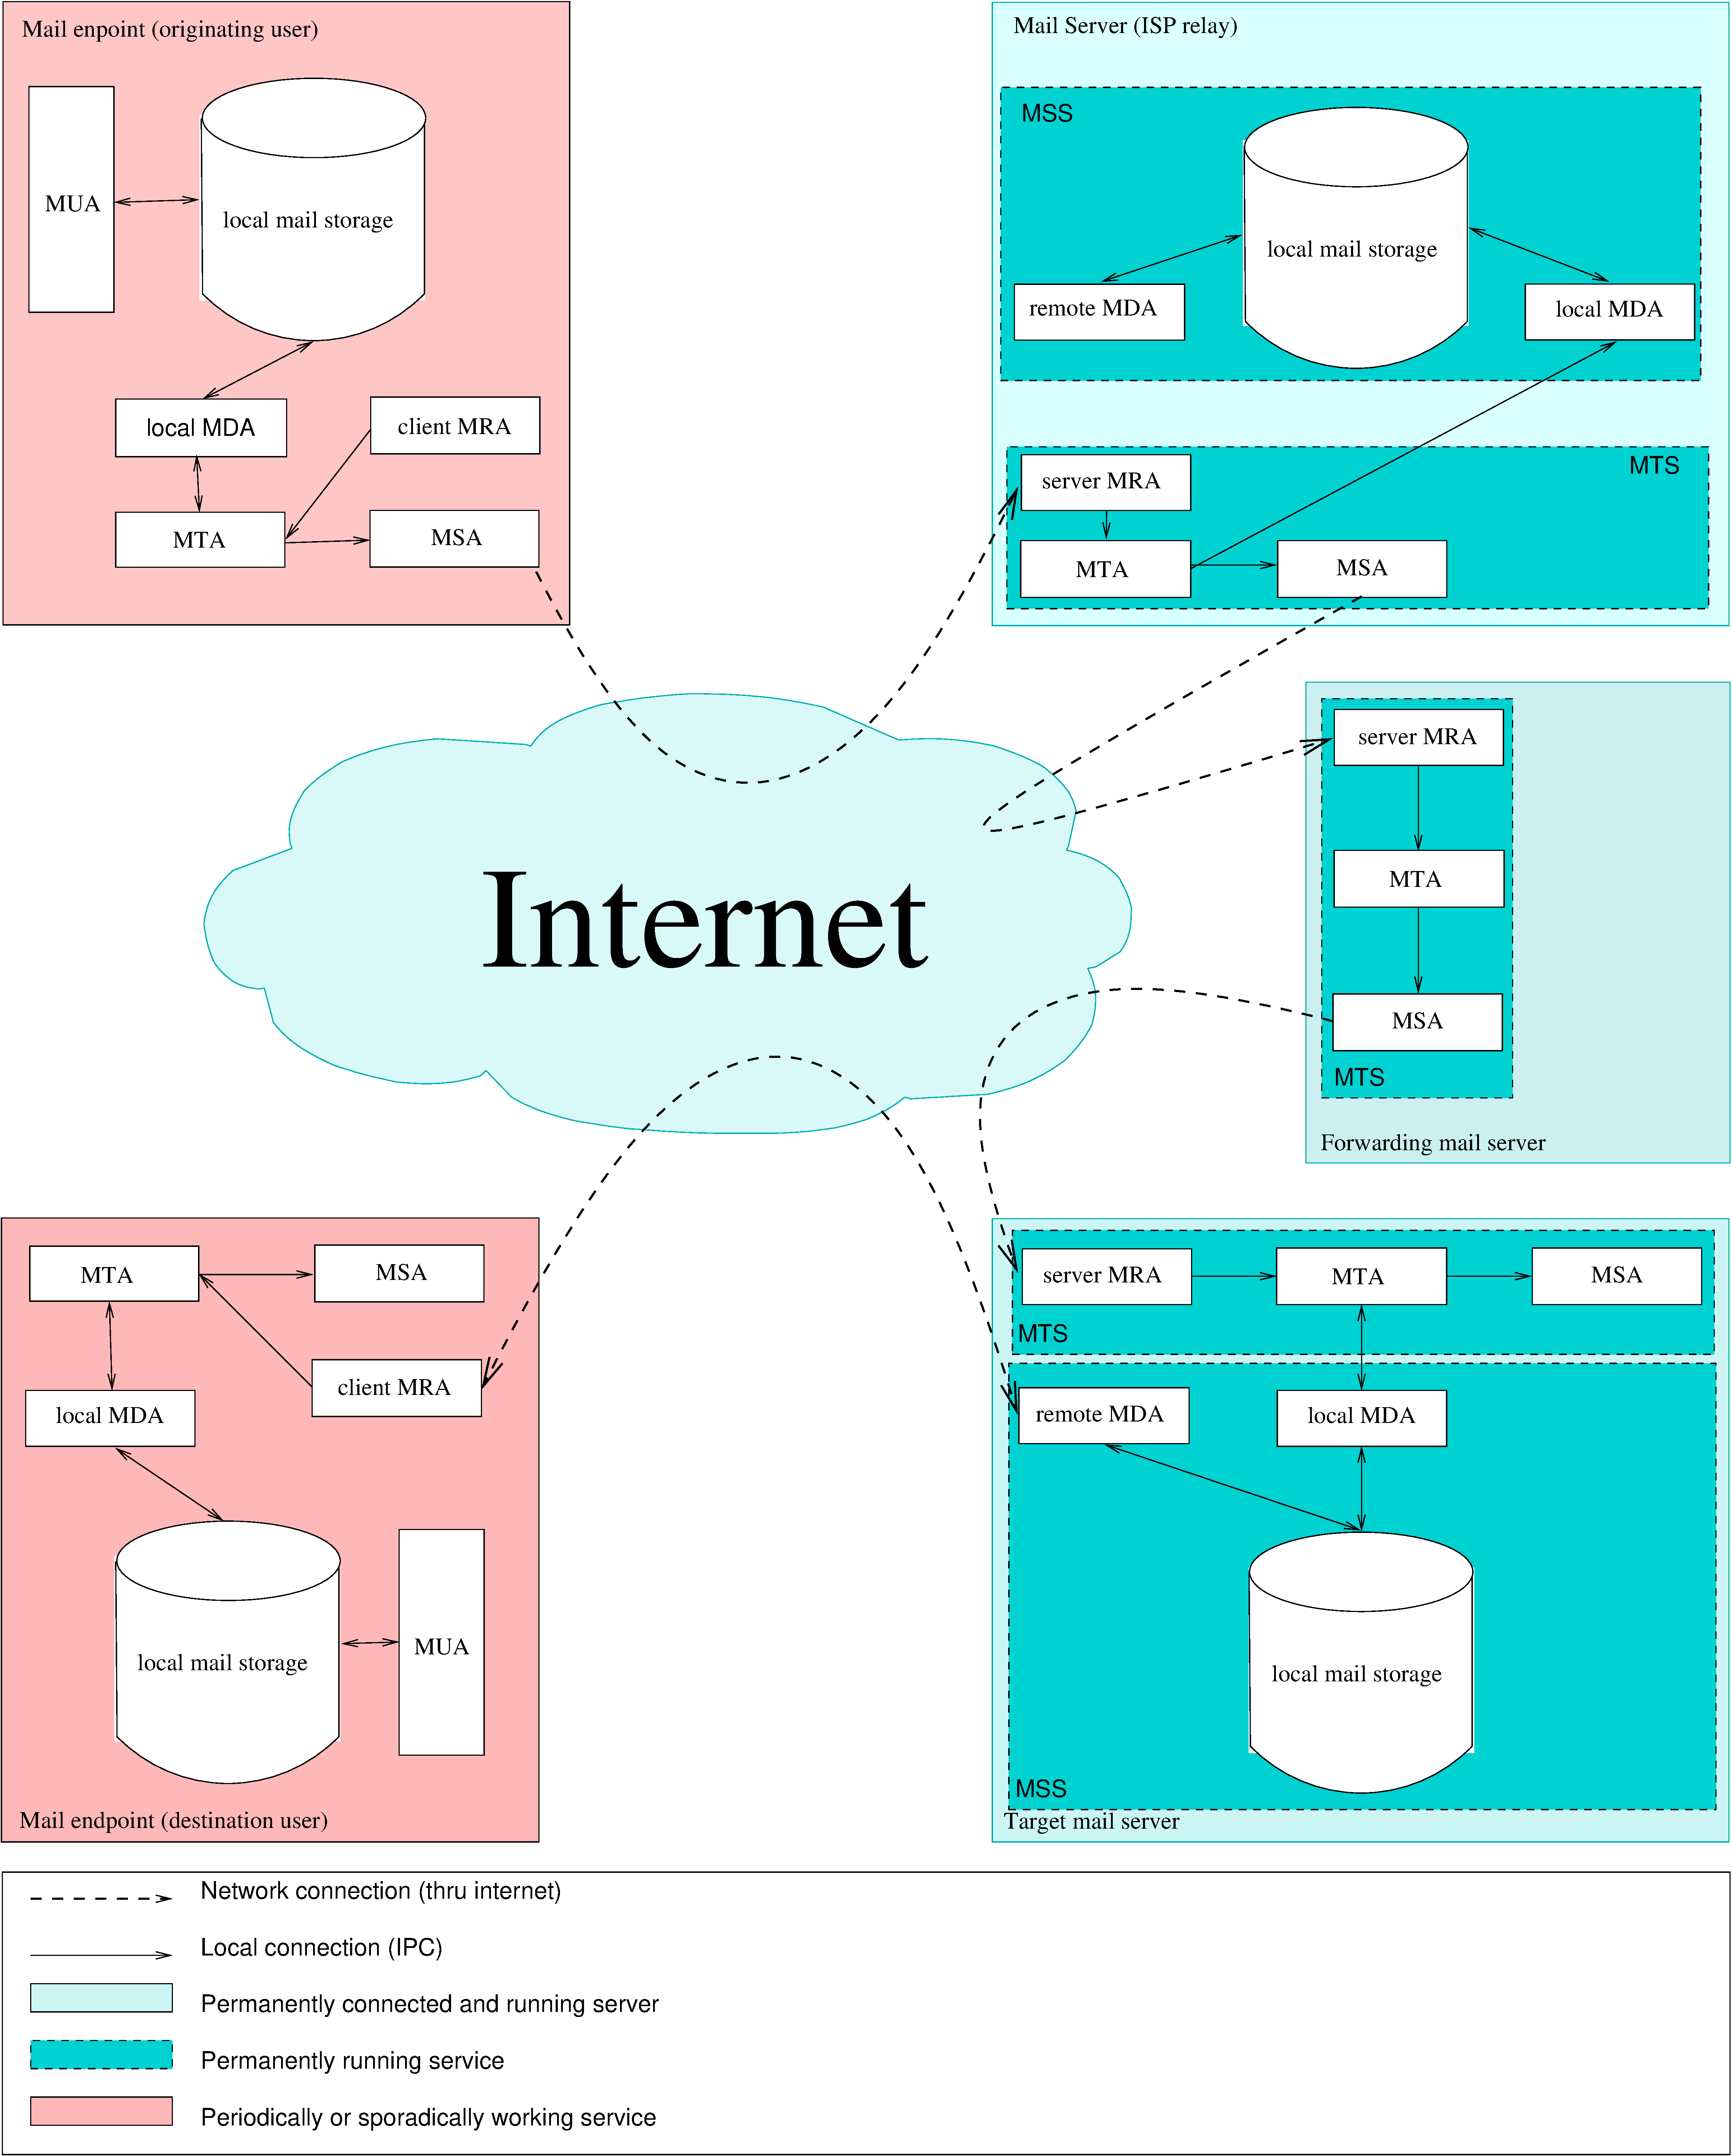
\includegraphics[width=\columnwidth]{inc/MailAgents1.pdf}
	\caption{Mail Agents}\label{fig:MailAgents}
\end{figure}

In the following paragraphs (for definitions), the term ``email'' is used synonymously to the term ``Message''.  ``Email'' has been chosen over ``messages'' because of its frequent use in standard documents.

Emails are typically initiated by a Mail User Agent (\defref{MUA}). An MUA accesses local email storage, which may be the server storage or a local copy. The local copy may be a cache only copy, the only existing storage (when emails are fetched and deleted from the server after retrieval), or a collected representation of multiple server storages (cache or authoritative).

Besides the MUA, the only other component accessing local email storage is the Mail Delivery Agent (\defref{MDA}). An MDA is responsible for storing and fetching emails from the local mail storage. Emails destined for other accounts than the current one are forwarded to the MTA. Emails destined to a User are persistently stored in the local email storage. It is essential to understand that email storage does not necessarily reflect a single mailbox. It may as well represent multiple mailboxes (e.g., a rich client-serving multiple IMAP accounts) or a combined view of multiple accounts (e.g., a rich client collecting mail from multiple \defref{POP} accounts). In the case of a rich client, the local MDA is part of the software provided by the user agent. In the case of an email server, the local MDA is part of the local email store (not necessarily of the mail transport service).

On the server-side, there are usually two components (services) at work. A ``Mail Transport Service'' (\defref{MTS}) responsible for mail transfers and a ``Mail Storage System'' which offers the possibility to store received Mails in a local, persistent store.\par

An MTS generally consists out of three parts. For incoming connects, there is a daemon called Mail Receiving Agent (\defref{Server MRA}) is typically a \defref{SMTP} listening daemon. A Mail Transfer Agent (\defref{MTA}) which is responsible for routing, forwarding, and rewriting emails. Moreover, a Mail Sending Agent (\defref{MSA}) which is responsible for transmitting emails reliably to another Server MRA (usually sent via \defref{SMTP}).\par

An MSS consists of local storage and delivery agents which do offer uniform interfaces to access the local store. They do also deal with replication issues, and grant should take care of the atomicity of transactions committed to the storage. Typically there are two different kinds of \defref{MDA}s. \defref{Local MDA}s offer possibilities to access the store via efficient (non-network based) mechanisms (e.g., IPC or named sockets). This is usually done with a stripped-down protocol (e.g., \defref{LMTP}). For remote agents there a publicly -- network-based -- agent available. Common Protocols for this \defref{Remote MDA}\ include \defref{POP}, \defref{IMAP}, or \defref{MS-OXCMAPIHTTP}.\par

\subsection{Email Endpoint Types}

Mail endpoints consist typically of the following components:
\begin{itemize}
	\item A Mail User agent (\defref{MUA})
	\item A Local Mail storage (\defref{MUA})
	\item A Local Mail Delivery Agent (\defref{Local MDA})
	\item A Mail Transfer Agent (\defref{MTA})
	\item A Mail Sending Agent (\defref{MSA})
	\item A Mail Receiving Agent (\defref{MRA})
\end{itemize}

Only two of these components do have external interfaces. These are \defref{MSA} and \defref{MRA}. \defref{MSA} usually uses \defref{SMTP} as transport protocol. When doing so, there are a couple of specialties. 
\begin{itemize}
	\item Port number is 587 (specified in \cite{RFC4409}).\\
	Although port numbers 25 and 465 are valid and do usually have the same capabilities, they are for mail routing between servers only. Mail endpoints should no longer use them.
	\item Connections are authenticated.\\
	Unlike a normal server-to-server (relay or final delivery) SMTP connections on port 25, clients should always be authenticated of some sort. This may be based on data provided by the user (e.g., username/password or certificate) or data identifying the sending system (e.g., IP address)\cite{RFC4409}. Failure in doing authentication may result in this port being misused as a sender for \defref{UBM}.
\end{itemize}

Mail User Agents (MUA) are the terminal endpoint of email delivery. Mail user agents may be implemented as fat clients on a desktop or mobile system or as an interface over a different generic protocol such as HTTP (Web Clients). 

Server located clients are a special breed of fat clients. These clients share the properties of fat clients except for the fact that they do not connect to the server. The client application itself has to be run on the server where the mail storage persists. This makes delivery and communication with the server different. Instead of interfacing with an MSA and a client MDA, they may directly access the local mail storage on the server. On these systems, the local mail storage may be implemented as a database in a user-specific directory structure.

\subsubsection{Fat clients}
The majority of mail clients are fat clients. These clients score over the more centralistic organized web clients in the way that they may offer mail availability even if an Internet connection is not available (through client-specific local mail storage). They furthermore provide the possibility to collect emails from multiple sources and store them in the local storage. Unlike Mail servers, clients are assumed to be not always online. They may be offline most of the time. To guarantee the availability of a particular email address, a responsible mail server for a specific address collects all emails (the \defref{MSS} does this) and provides a consolidated view onto the database when a client connects through a local or remote MDA.

As these clients vary heavily, it is mandatory for the MDA that they are well specified. Lack of doing so would result in massive interoperability problems. Most commonly the Protocols \defref{IMAP}, \defref{POP} and \defref{EWS} are being used these days. For email delivery, the SMTP protocol is used. 

Fat clients are commonly used on mobile devices. According to  \cite{clientDistribution} in Aug 2012 the most typical fat email client was Apple Mail client on iOS devices ($35.6\%$), followed by Outlook ($20.14\%$), and Apple Mail ($11\%$). \citetitle{clientDistribution2}\cite{clientDistribution2} as a more recent source lists in February 2014 iOS devices with $37\%$, followed by Outlook ($13\%$), and  Google Android ($9\%$).

\subsubsection{Server located clients}
Server located clients build an absolute minority. This kind of clients was common in the days of centralized hosts. An example for a Server Located Client is the Unix command ``mail''. This client reads email storage from a file in the users home directory.

\subsubsection{Web clients}
Web clients are these days a common alternative to fat clients. Most big provider companies use their proprietary web client. According to \cite{clientDistribution2} the most common web clients are "`Gmail"', "`Outlook.com"', and "`Yahoo! Mail"'. All these Interfaces do not offer a kind of public plug-in interface. However,  they do offer IMAP-interfaces. This important for a future generalistic approach to the problem.

\subsection{S/MIME}
S/MIME is an extension to the MIME standard. The MIME standard allows in simple text-oriented mails an alternate representation of the same content (e.g., as text and as HTML), or it allows to split a message into multiple parts that may be encoded. It is important to note that MIME encoding is only effective in the body part of an mail.

S/MIME, as described in \cite{RFC3851}, extends this standard with the possibility to encrypt mail content or to sign it. Practically this is achieved by either putting the encrypted part or the signature into an attachment. It is essential to know that this method leaks significant pieces of the data.

As the mail travels directly from sender to recipient, both involved parties are revealed. Neither message subject nor message size or frequency is hidden. This method does offer limited protection when assuming an adversary with interest in the message content only. It does not protect from the kind of adversary in our case. 

The trust model is based on a centralistic approach involving generally trusted root certification authorities.

\subsection{PGP/MIME}
Exactly as S/MIME PGP\cite{rfc4880} builds upon the base of MIME. Although the trust model in PGP is peer-based. The encryption technology does not significantly differ (as seen from the security model).

Like S/MIME, PGP does not offer anonymity. Sender and endpoints are known to all routing nodes. Depending on the version of PGP, some meta-information or parts of the message content such as subject line, the real name of the sender and receiver, message size is leaked.

A good thing to learn from PGP is that peer-based approaches are offering limited possibilities for trust. The trust in PGP is based on the peer review of users. This peer review may give an idea of how well verified the key of a user is.


\section{Pseudo Random Number Generators \label{sec:prng}}
The following sections list two PRNG specifications to follow the recommendations of \cite{rfc1750}. These PRNGs are used to complete the padding specified in the addRedundancy operation.

We have chosen to support two kinds of PRNG. These algorithms are not relevant for the security of the system, but they guarantee non-detectable padding when doing the addRedundancy operation. The two PRNGs selected were xorshift128+ and Blum Micail PRNG. Both PRNGs were quoted to pass BigCrush. However, recent development shows that this might not be true for xorshift128+, as demonstrated in \cite{LEMIRE2019139}.

\section{Known Attacks}
In the following sections, we emphasize on possible attacks to an anonymity preserving protocols. These attacks may be used to attack the anonymity of any entity involved in the message channel. In a later stage, we test the protocol for immunity against these classes of attacks.

\subsection{Broken Encryption Algorithms}
Encryption algorithms may become broken at any time. This either to new findings in attacking them, by more resources being available to an adversary, or by new technologies allowing new kinds of attacks. A proper protocol must be able to react to such threads promptly. This reaction should not rely on a required update of the infrastructure. Users should solely control the grade of security. 

We cannot do a lot for attacks of this kind to happen. However, we might introduce a choice of algorithms, paddings, modes, and key sizes to give the user a choice in the degree of security he wants to have.

\subsection{Attacks Targeting Anonymity}
Attacks targeting users anonymity are the main focus of this work. Many pieces of information may be leaked, and the primary goal should, therefore, rely on the principles established in security.

\begin{itemize}
	\item Prevent an attack\\
	Attack prevention can only be done for attacks that are already known and may not be realistic in all cases. In our protocol, we have strict boundaries defined. A node under attack should at any time of protocol usage (this excepts bandwidth depletion attacks) be able to block malicious identities. Since establishing new identities is costly for an attacker, he should always require far more resources than the defender.
	\item Minimize attack surface\\
	This part of the attack prevention is included by design in the protocol.
	\item Redirect an attack\\
	Although the implementation does not do this, it is possible to handle suspected malicious nodes differently.
	\item Control damage\\
	For us, this means leaving as little information about identities or meta information as possible on untrusted infrastructures. If we leave traces (i.e., message flows, or accounting information) they should have the least possible information content and should expire within a reasonable amount of time.
	\item Discover an attack\\
	The protocol is designed in such a way that attack discovery (such as a query attack) is possible. However, we consider active attacks just as part of the regular message flow. The protocol must mitigate such attacks by design.
	\item Recover from an attack\\
	An attack does always impose a load onto a system's resources regardless of its success. It is vital that a system recovers almost immediately from an attack and is not covered in a non-functional or only partial-functional state either temporarily or permanently.
\end{itemize}

In the following subsections, we list a couple of attack classes that have been used against systems listed in \ref{sec:sysImpl} or the respective academic works. We list the countermeasures which have been taken to deflect these attacks.

\subsubsection{Probing Attacks}
Identifying a node by probing and check their reaction is commonly done when fingerprinting a service. As a node is participating in a network and relaying messages probing may not be evaded. However, it may be made costly for an adversary to do systematic probing. This should be taken into account. Both currently specified transport protocol features an indefinite number of possible accounts. Since not the server but the endpoint address is behaving, node probing is more complicated than in other cases where probing of service is sufficient. 

One of the problems is clear-text requests. These requests may be used on any transport layer account without previous knowledge of any host key. Thus the recommendation in table \ref{tab:protoReplyCrit} is generally not to answer the requests. Routing nodes in jurisdictions not fearing legal repression or prosecution may reply to clear text requests, but it is usually discouraged as they allow harvesting of addresses.

One strategy to avoid would be to put high costs onto clear-text requests in such a way that a clear-text request may have a long reply time (e.g., up to one day). A node is free to blacklist an identity in case of an early reply. This is an insufficient strategy as a big adversary may have lots of identities in stock. Requesting an unusually long key as a plain-text identity does not make sense either as these as well may be kept in stock. We may, however, force a plaintext request to have an identity block with a hash following specific rules. We may, for example, put in a requirement that the first four bytes of the hash of a header block translate to the first four characters of the routing block. At the moment, this has been rejected in the standard for practical reasons. First, as the request is unsolicited, a sender is the only one able to decide the algorithm of the hash. This would allow a requester to choose upon the complexity of the puzzle. Second, any negotiation of the cost of the request would result in the disclosure of the node as VortexNode, which might be unsuitable.

\subsubsection{Hotspot Attacks}
Hotspot attacks aim to isolate high traffic sites within a network. By analyzing specific properties or the general throughput locations with outstanding traffic may be identified. These messages do quite often reveal senders or recipients. Sometimes an intermediate node in an anonymizing system. 

\subsubsection{Message Tagging and Tracing}
When using an anonymization system, a message may be either fully or partially traced or even tagged. Tagging allows one to recognize a message at a later stage and map it to its predecessors. Protocols with tagable messages are not suitable for anonymization systems.

\subsubsection{Side Channel Attacks}
Side-channel attacks are numerous. Especially important to us are attacks related to either lookup in independent channels (e.g., downloading of auxiliary content of a message) or behavior related to timing patterns.

\subsubsection{Sizing Attacks}
There are two kinds of sizing attacks identified to be relevant for us. One is the possibility for matching messages with related sizes, and the other one is to relate message size to the original messages. Both attacks may be considered as a tracing attack and will be analyzed accordingly.

\subsubsection{Bugging Attacks}
Numerous attacks are available through the bugging of a protocol. In this chapter, we outline some of the possibilities and how they may be countered:

\begin{itemize}
	\item Bugging through certificate or identity lookup:\\
	Almost all kinds of proof of identities, such as certificates, offer some revocation facility. While this is a perfect desirable property of these infrastructures, they offer a flaw. Since the location of this revocation information is typically embedded in the proof of identity, an evil attacker might use a falsified proof of identity with a recording revocation point.
	
	There are multiple possibilities to counter such an attack. The easiest one is to do no verification at all. Having no verification is, however, not desirable from the security point of view. Another possibility is only to verify trusted proof of identities. By doing so, the only attacker could be someone having access to a trusted source of proof of identities. A third possibility is to relay the request to another host either by using an anonymity structure such as Tor or by using its infrastructure. Using Tor would violate the ``Zero Trust'' goal. Such a measure would only conceal the source of the verification. It would not hide the fact that the message is processed. A fourth and most promising technology would be to force the sender of the certificate to include a ``proof of non-revocation''. Such a proof could be a timestamped and signed partial CRL. It would allow a node to verify the validity of a certificate without being forced to disclose itself by doing a verification. On the downside has to be mentioned that including proof of non-revocation involves the requirement to accept a certain amount of caching time to be accepted. This allowed caching time reduces the value of the proof as it may be expired in the meantime. It is recommended to keep the maximum cache time as low as 1d to avoid that revoked certificates may be used. 
	
	\item Bugging through DNS traffic:\\
	A standard protocol on the Internet is DNS. Almost all network-related programs use it without thinking. Typically the use of such protocol is only a minor issue since the resolution of a lookup usually done by an ISP. In the case of a small Internet service provider (ISP), this might, however, already become a problem.
	
	The bugging in general attack works as follows: We include a unique DNS name to be resolved by a recipient. This can be done most easily by adding an external resource such as an image. A recipient will process this resource and might, therefore, deliver information about the frequency of reading, or the type of client. 
	
	It must be taken into account that the transport layer will always do DNS lookups and that we may not avoid this attack completely. We may, however, minimize the possibilities of this attack.
	
	\item Bugging through external resources:\\
	A straightforward attack is always to include external resources into a message and wait until they are fetched. In order to avoid this kind of attack, plain text or other self-contained formats should be used when sending a message. As we may not govern the type of contained message, we can make at least recommendations concerning its structure.
\end{itemize}

\subsection{Denial of Service Attacks}
\subsubsection{Censorship}
Whereas traditional censorship is widely regarded as selective information filtering and alteration, very repressive censorship can even include denial of information flows in general. Any anonymity system not offering the possibility to hide in legitimate information flows, therefore not censorship-resistant.

\subsubsection{Denial of service}
An adversary may flood the system in two ways.
\begin{itemize}
	\item He may flood the transport layer exhausting resources of the transport system.\\
	This is a straightforward attack. MessageVortex has no control over the existing transport protocol. Therefore, all flooding attacks on that layer are still effective. However, If an adversary attacks a node, the redundancy of a message may still be sufficient. On the other hand, flooding disrupts at least all other services using the same transport layer on that node. This result may be unacceptable for an attacker. More likely would be censorship.
	\item He may flood the routing layer with invalid messages.\\ 
	Identifying the messages is relatively easy for a node. Usually, it should be sufficient to decode the CPREFIX block of a message. If the CPREFIX is valid, then the header block either identifies a valid identity or processing may be aborted. 
	\item He may flood an accounting layer with newIdentity.\\
	Flooding an accounting layer with identities is possible. Since the accounting layer is capable of adapting costs to a new identity, it may counter this attack by giving large puzzles to new identities. This affects all new identities and not only those flooding. If a flooding attack is carried out over a long time, a node may decide to split its identity. All recent active users get a new identity, whereas the old one opposes high costs. This would force an attacker to work in intervals and is no longer able to make a permanent DoS attack.
\end{itemize}

\subsubsection{Credibility Attack}
Another type of DoS attack is the credibility attack. While not a technical attack, it is very effective. A system not having a sufficiently big user base is offering thus a lousy level of anonymity because the anonymity set is too small or the traffic concealing message flow is insufficient. 

Another way is to attack the reputation of a system in such a way that the system is no longer used. An adversary has many options to achieve such a reduction in credibility. Examples:
\begin{itemize}
	\item Disrupt functionality of a system.\\ 
	This may be done by blocking of the messaging protocol it uses or by blocking messages. Furthermore, an adversary reduces functionality when removing known participants from the network either by law or by threatening.
	\item Publicly dispute the effectiveness of a system.\\
	Disputing the effectiveness is a very effective way to destroy a system. People are not willing to use a system which believed to be compromised if the primary goal of using the system is avoiding being observed.
	\item Reduce the effectiveness of a system.\\
	A system may be considerably loaded by an adversary to decrease the positive reception of the system. He may further use the system to send \defref{UBM} to reduce the overall experience when using the system. Another way of reducing effectiveness is to misuse the system for evil purposes such as blackmailing and making them public.
	\item Dispute the credibility of the system founders.\\
	Another way of reducing the credibility of a system is to undermine its creators. If -- for example -- people believe that a founders' interest was to create a honey pot (e.g., because he is working for a potential state-sponsored adversary) for personal secrets, they will not be willing to use it.
	\item Dispute the credibility of the infrastructure.\\
	If the infrastructure is known or suspected to be run by a potential adversary, people's willingness to believe in such a system is expected to be drastically reduced.
\end{itemize}

\chapter{Applied Methodes\label{sec:appliedMethods}}
Based on the findings of the previous chapter, we used the following methodology in order to find a solution:
\begin{enumerate}
	\item Identify problem hotspots for a new protocol.
	\item Design a protocol that addresses the previously identified hotspots.
	\item Build a protocol prototype.
	\item Analyse the protocol for weaknesses using attack schemes.
	\begin{enumerate}
		\item Tagging/Bugging attacks.
		\item Tracing attacks.
		\item Content and identification targeting attacks.
		\item DoS attacks.
	\end{enumerate}
\end{enumerate}

\section{Problem Hotspots}
Starting from the previous research, we identified several hotspots that have to be taken care of. The following sections list identified problems and the possible countermeasures which have not been broken in the past.

\subsection{Zero Trust Philosophy}
One main disadvantage of almost any system listed in section \ref{sec:sysImpl} is that trust (unlimited or limited) has been put into the infrastructure. For example, when using ToR, we need to trust the directory servers. Control over the directory servers might give an attacker the possibility to redirect a connection to controlled entry and exit nodes, which would then break anonymity. In general, control of entry and exit nodes makes a system vulnerable. 

To avoid this problem, we decided to apply a zero trust model. We do not trust any platform except for the sending and the receiving computer. We assume that all other devices may be compromised and do create detailed logs about what they are doing. This trust extends partially to our personally known contacts. We believe that some of them might be evil, but they are generally trustworthy. We furthermore assume that traffic on the network layer is observed and recorded at any time. This philosophy creates very hard to meet goals. However, by assuming so, we prevent the system from leaking information through side channels.

\begin{requirement}{zeroTrust}{Zero Trust}
	No infrastructure should be trusted unless it is the senders' or the recipients' infrastructure.
\end{requirement}    

\subsection{Information leakage and P2P Design}
An anonymizing system must keep information on messages or their metadata within the system. Ideally, even not disclosing to its members. In a perfectly encrypted system, such metadata is leaked at least by the entry and the exit node. To avoid this, all peers must behave alike. All nodes should be valid endpoints as well as legitimate senders or mixes. Covering all functions in all nodes implies a design with equally built nodes and is shared with many P2P designs.

A fundamental problem of the P2P design is that usually, port forwarding or central infrastructure is required. Technologies such as ``hole punching'' and ``hairpin translation'' typically require central infrastructures to support at least the connection and maybe depending on the client infrastructure being used fragile or ineffective. To avoid these problems we decided to rely on traditional centralistic transport infrastructures. As proof of concept, we decided to use SMTP. 

The approach supports, however, even mixing transport media. This makes it harder for an attacker to trace a message as the message flow may go through any suitable transport protocol at any time of message transfer.

\begin{requirement}{P2P}{Equal nodes}
	Mixes and peers must be indistinguishable from each other. 
\end{requirement}

\subsubsection{Decoy traffic generation}
To create decoy traffic in an untrusted way, we need means to increase and decrease messages in size without knowledge of the routing node. A straightforward approach would be to create decoy traffic in the initial message. Such a design would create a pattern of decreasing or repeating message sizes in the net. To avoid this, we introduced a set of operations to be applied to the original message. The operations are done in such a way that a mixer is unable to tell whether the message size or decrease results in decoy traffic generation/removal or not.

The main message operations are:
\begin{itemize}
	\item Split and merge messages.
	\item Add and remove redundancy information.
	\item Encrypt and Decrypt information.
\end{itemize}

At this point, we could have used homomorphic encryption instead of redundancy operations. Such encryption would, however, add much complexity to the algorithm with no apparent gain.

\subsubsection{Message tagging or bugging protection}
It is essential to the protocol that any operation at any point of the protocol handling, which is not foreseen, should fail in message transport. This property makes the protocol very fragile, but it prevents mixes from introducing tags which may be followed throughout the system. The protocols counter this fragility by the fact that redundancy added in the message course may be used to recover from misbehaving nodes.

In our approach, we give a single mix called the routing block builder (RBB) full control over the message transport layer. The content used for blending is discardable data. RBB has no control over this aspect. This blending data is ephemeral and will (or may) be removed by the next node. The data received by a mix may be used to generate a ``pseudo reply'' on the blending layer to transport any other message (related or unrelated) back to the sending node. So tagging on this layer is worthless.

The reason for not giving control over the behavior to this layer to the sender of the message is simple. By giving him control over it, we would allow him to use the information provided here as the primary medium. As an immediate result, the system would be suitable to blackmail any user of the world. It furthermore would create unintentional ``exit nodes'' to the system, which might oppose further legal threads for participants.

\begin{requirement}{untagable}{untagable}
	The message should be un-tagable (neither by a sender nor by an intermediate party such as a mixer).
\end{requirement}

\begin{requirement}{unbugable}{unbugable}
	The message should be unbugable (neither by the sender nor by an intermediate party such as a mixer).
\end{requirement}

\subsubsection{Message replay protection}
Message reply protection is crucial for such a system. With the ability to replay a message, an adversary may ``highlight'' a message flow as it would always generate the same traffic pattern. So there needs to be a reply pattern protecting the protocol from message replay. As we do have MURBs in our protocol, this is a problem. A MURB is by design replayable. We, therefore, need a possibility for the original sender using a MURB to make messages distinguishable, which may not be used by an adversary.

\begin{requirement}{replay}{replay}
	A message must not be replayable.
\end{requirement}

It should be able to increase and shrink in size, or all messages must have a uniform size. Decoy traffic should not be distinguishable from message traffic. 

\subsubsection{No Dedicated Infrastructure Philosophy}
There should be no infrastructure dedicated to the operation of the solution. This avoids a single point of failure, as well as the possibility for an adversary to shut down this infrastructure to disrupt the functioning of the system as a whole. This requirement is already covered implicitly in \ref{req:zeroTrust}.

\subsection{Accounting}
The infrastructure must not be misused as \defref{UBM} sending infrastructure. This implies that sending messages is connected to some ``cost''. ``Costs'' must be connected to some identity to allow accounting. Linking to a global identity would allow assigning traffic to a real-world user. Therefore the protocol must allow creating ephemeral local identities not linked to a real identity.

\begin{requirement}{accounting}{accounting}
	The system must be able to do accounting without being linked to a real identity.
\end{requirement}

\subsection{Anonymisation}
The system must allow the anonymizing of message source and message destination at any point. It should not be visible to the infrastructure protocol whether a message has reached its destination or not. 

\begin{requirement}{anon}{anonymisation}
	A system must be able to anonymize sender and recipient at any point of the transport layer and any point of mixing unless it is the sender or the recipient itself.
\end{requirement}

\subsection{Initial Bootstraping}
The system must allow bootstrapping from a zero-knowledge or near-zero knowledge point. Therefore, the protocol must be able to extend the network of known nodes on its own.

\begin{requirement}{boot}{bootstrapping}
	The system must allow to bootstrap from a zero-knowledge or near-zero-knowledge point and extend the network on its own. 
\end{requirement}

\subsection{Cypher selection}
In this protocol, a lot of encryption and hashing algorithms have to be used. This choice of these algorithms should be explained. 

From the requirements side, we have to follow the following principle:
\begin{requirement}{algVar}{algorithmic variety}
	The system must be able to use multiple symmetric, asymmetric, and hashing algorithms to immediately fall back to a secure algorithm for all new messages if required. 
\end{requirement}

First of all, we need a subset of encryption algorithms all implementations may rely on. Defining such a subset guarantees interoperability between all nodes regardless of their origins. 

Secondly, we need to have a spectrum of algorithm in such a manner that it may be (a) enlarged if necessary and (b) there is an alternative if an algorithm (or a mathematical problem class) is broken (so that algorithms may be withdrawn if required without affecting the function in general). 

And third, due to the onion-like design described in this document, asymmetric encryption should be avoided in favor of symmetric encryption to minimize losses due to the key length and the generally higher CPU load opposed by asymmetric keys.

If the algorithm is generally bound to specific key sizes (due to S-Boxes or similar constructs), the key size is incorporated into the definition. If not, the key size is handled as a parameter.

The key sizes have been chosen in such a manner that the key types form tuples of approximately equal strength. The support of Camelia192 and Aes192 has been defined as optional. However, as they are wildly common in implementations, they have already been standardized as they build a possibility to step up security in the future.

Having these criteria for choice, we chose to use the following keys and key sizes:
\begin{itemize}
	\item Symmetric
	\begin{itemize}
		\item AES (key sizes: 128, 192, 256)
		\item Camellia (key sizes: 128, 192, and 256)
	\end{itemize}
	\item Asymmetric
	\begin{itemize}
		\item RSA (key size: 2048, 4096, and 8192)
		\item Named Elliptic Curves
		\begin{itemize}
			\item secp384r1
			\item sect409k1
			\item secp521r1
		\end{itemize}
	\end{itemize}
	\item Hashing
	\begin{itemize}
		\item sha3-256
		\item sha3-384
		\item sha3-512
		\item RIPE-MD160
		\item RIPE-MD256
		\item RIPE-MD320
	\end{itemize}
\end{itemize}

Within the implementation, we assigned algorithms to a security strength level:
\begin{itemize}
	\item LOW\\
	AES128, Camellia128, RSA1024, sha3-256
	\item MEDIUM\\
	AES192, Camellia 192, RSA2048, ECC secp384r1, sha3-256
	\item HIGH\\
	AES256, Camellia256, RSA4096, ECC sect409k1, sha3-384
	\item QUANTUM\\
	AES256, Camellia256, RSA8192, ECC secp521r1, ntru, sha3-512
\end{itemize}

This allows categorizing the used algorithms to a strength. This list, however, should only serve the purpose of selecting algorithms for people without cryptological know-how.

\subsection{Reed-Solomon function}
Originally \cite{reed1960polynomial} introduced a system allowing the use of polynomial codes to create error-correcting codes. In \cite{chaum1988multiparty} \citeauthor{chaum1988multiparty}, they have shown that the codes are suitable for distributing data assuming enough parties are honest.

Unlike Chaum et al., we are not using the Reed Solomon function to achieve anonymity or privacy. Instead, we use it for decoy traffic generation. We are splitting a message into multiple parts at several points when routing and assemble it again on different nodes. By doing so, we achieve two vital things. First, we introduce the possibility of recovering errors due to misbehaving nodes, and secondly, the real traffic can no longer be differentiated from decoy traffic. 

\subsection{Usability}
The system must be usable without cryptographic know-how and with popular tools. This is necessary to accept the system broadly and makes it easy to use for peoples already communicating.

\begin{requirement}{easy}{easy handleable}
	The system must be usable without cryptographic know-how and with popular tools.
\end{requirement}

\section{Protocol outline}
The protocol itself is independent of the transport layer specified. We emphasize in this section to the general building blocks, the cryptographic structure, and the general protocol attributes. In section \ref{sec:spec}, we will then further elaborate on the protocols' inner structure.

The protocol is built on multiple layers. On the logic side, the protocol is split into two parts:
\begin{enumerate}
	\item Transport Layer\\
	Standard Internet infrastructures provide this Layer. The primary goal is to hide or blend our protocol into regular traffic within that layer.
	\item Blending and subsequent layers\\
	Any user of the Internet may provide these layers. Since these layers may be mixes-only, or valid endpoints. Mixes may or may not be publicly known. In a first implementation, we build this system as a standard Java application. The primary goal is to compile it to native code afterward and run it on an SoC like infrastructure such as a RaspberryPi or port it to an android device.
	
	We may further split these layers into
	\begin{enumerate}
		\item Blending layer\\
		This layer takes messages and creates transport layer conformant messages. In an ideal case, the messages generated by this layer are indistinguishable from the regular message traffic, and the embedded message is only visible for the receiving node.
		\item Routing layer\\
		The routing layer disassembles and reassembles messages. This operation guarantees that messages are generated in such a way that decoy traffic is not differentiable from non-decoy traffic.
		\item Accounting layer\\
		The accounting layer has three jobs. First, he has to authorize the message processing after decrypting the header block. Secondly, he handles all header request blocks and the reply blocks. And third, it keeps track of the accounting regarding the sent messages.    
	\end{enumerate}
\end{enumerate}

%%%%%%%%%%%%%%%%%%%%%%%%%%%%%%%%%%%%%%%%%%%%%%%%%%%%%%%%%%%%%%%%%%%%%%%%%%%%%%%%%%%%%%%
% revise from this point on %%%%%%%%%%%%%%%%%%%%%%%%%%%%%%%%%%%%%%%%%%%%%%%%%%%%%%%%%%%
%%%%%%%%%%%%%%%%%%%%%%%%%%%%%%%%%%%%%%%%%%%%%%%%%%%%%%%%%%%%%%%%%%%%%%%%%%%%%%%%%%%%%%%

\subsection{Protocol Terminology}
For our protocol, we use the following terms:
\begin{itemize}
	\item \textbf{Sender:} The user or process originally composing the message.
	\item \textbf{Recipient:} The user or process destined to receive the message in the end.
	\item \textbf{Router:} Any node which is processing the message. Please note that all nodes are routers.
	\item \textbf{Message:} The ``real content'' to be transferred from the sender to the recipient.
	\item \textbf{Payload:} Any data transported between routers regardless of the meaningfulness or relevance to the message.
	\item \textbf{Decoy traffic:} Any data transported between routers that have no relevance to the message at the final destination.
	\item \textbf{Identity:} A tuple of a routable address, and a public key. This tuple is a long-living tuple but may be exchanged from time to time. 
	\item \textbf{Ephemeral Identity:} An identity created on any node with a limited lifetime anyone possessing the private key (proven by encrypting with it) is accepted as representative of that identity.
	\item \textbf{Routing Block Builder (RBB):} An entity, which is building a routing block. Typically identical to either sender or receiver.
\end{itemize}

\subsection{Vortex Communication model}
In this section, we introduce a new consistent, transport-independent model for representing the different protocols used by MessageVortex.

\begin{figure}[ht!]
	\centering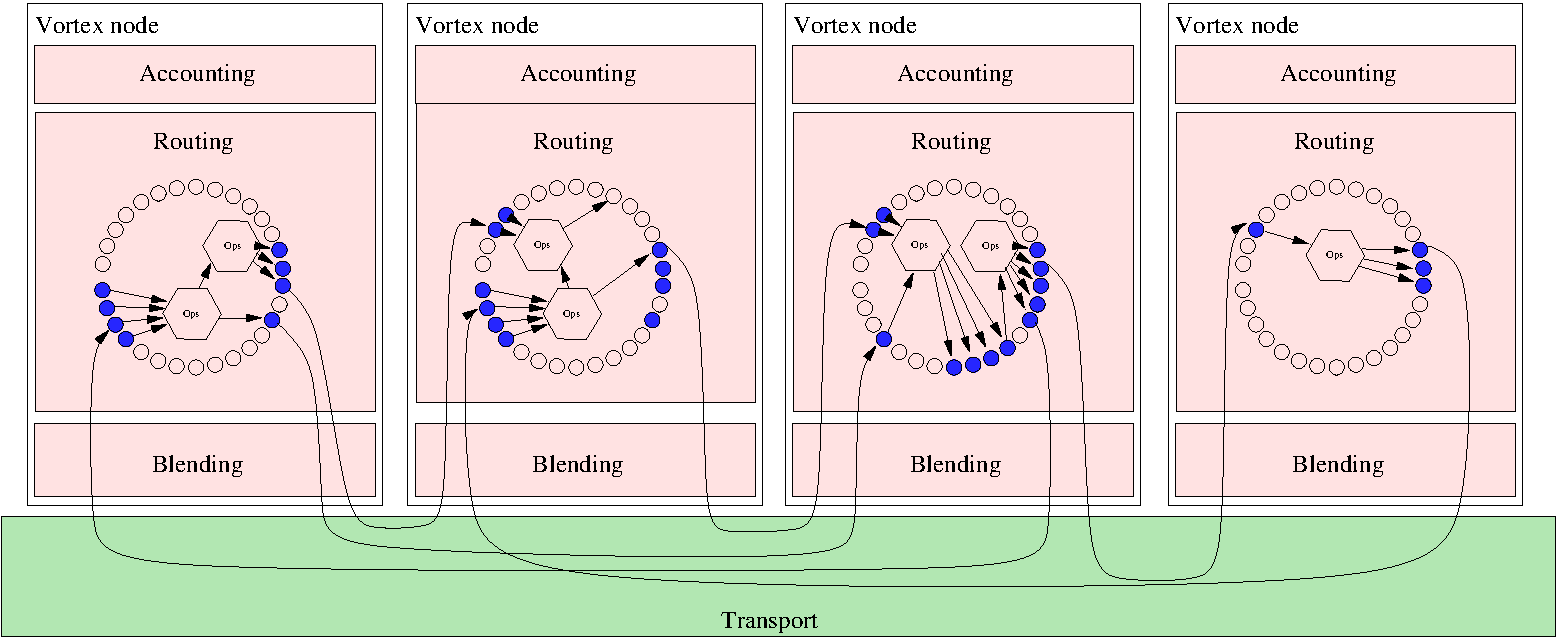
\includegraphics[width=\columnwidth]{inc/roughProtocolDesign.pdf}
	\caption{A rough protocol outline of the MessageVortex protocol}\label{fig:protocolOutline}
\end{figure}

We divide our protocol into four different layers, whereas only three are specific to the MessageVortex protocol. The lowest layer is the transport layer. As expressed earlier, dedicated protocols are easy to censor. Therefore we build our protocol on top of other suitable transport protocols. 

The other Three layers are vortex specific and do not require any infrastructure on the Internet. We elaborate further on these layers in the next section.

\subsection{Transport Layer}
For our first tests, we used a custom transport layer, allowing us to monitor all traffic quickly, and build structures in a very flexible way. This transport layer works locally with a minimum amount of work for setup and deployment. It furthermore works across multiple hosts in a broadcast domain. The API may be used to support almost any kind of transport layer.

After that, we focussed on the protocols identified in the previous sections for transport:
\begin{itemize}
	\item SMTP
	\item XMPP
\end{itemize}
For the prototype, we have implemented an SMTP transport agent and the respective blending layer.

\subsection{Blending Layer}
The blending layer is taking care of multiple problems:
\begin{itemize}
	\item It is translating the message block into a suitable format for transport\\
	This translation includes jobs such as embedding a block as encoded text, as a binary attachment or hide it within a message using steganography.
	\item Extract incoming blocks\\
	Identify incoming messages containing a possible block and extract it from the message.
	\item Do housekeeping on the storage layer of the transport protocol\\
	Access protocols POP and IMAP require that messages are deleted from time to time to stay below the sizing quotas of an account.      
\end{itemize}

We define the blending layer to work as follows when receiving messages:

\begin{enumerate}
	\item Log arrival time (in UTC) on the transport layer.
	\item Extract possible blocks.
	\item Apply decryption on a suspected header block.
	\item Identify the header block as valid by querying the accounting.
	\item Extract and decrypt subsequent blocks.
	\item Pass extracted blocks and information to the routing layer.
\end{enumerate}

We define the blending layer to work as follows for sending messages:

\begin{enumerate}
	\item Assemble message as passed on by the routing layer.
	\item Using the blending method specified in the routing block, build an empty message. 
	\item Create a message decoy content.
	\item Send the message to the appropriate recipient using the transport layer protocol.
\end{enumerate}

There is no specification on the housekeeping part of the blending layer, as this part is specific to the requirements of the account owner. We do, however, recommend to handle messages precisely as if the messages would be handled on an account handled by a human. 

\subsection{Routing Layer}
The routing layer receives the message blocks in a decrypted and authorized form from the blending layer and processes them as follows:

\begin{itemize}
	\item Build structure representing the block building and the appropriate block IDs.
	\item Schedule all Routing blocks for processing in a priority queue.
	\item Authorise all routing blocks ready for processing with the calculated block sizes.
	\item Process blocks.
	\item Send prepared building blocks to the Blending layer.
\end{itemize}

\subsubsection{Block Structure}
A VortexMessages' main block structure is a sequence of blocks. This block sequence starts with a header containing a symmetric key encrypted with the public key of the current node and a header block containing the immediate details to decrypt the subsequent blocks (if any).

A routing block follows the header block. This routing block contains the information required for subsequent routing. According to the instructions in this block, valid data blocks may be processed, assembled, and sent to a subsequent location. 

The next block is the routing log block. This block protocols the routing information of a message and is somewhat similar to an onionized variant of the received headers in SMTP.

The last part of the message is a sequence of data blocks. They contain the actual data or decoy traffic.

\subsubsection{MURBs\label{sec:murb}}
The protocol includes the capability of MURBs. Such MURBs enable a user to send a limited amount of times messages to an anonymous receiver. Such sending may be done without having any knowledge about its identity, the location, or infrastructure he is using.

A MURB in our term is an entirely prepared routing instruction built by the recipient of a message. The sender has only the routing blocks and the instructions to assemble the initial message. It does not know the message path except for the first message hops.

As a MURB is a routing block, it generates the same pattern on the network each time a sender uses it. To avoid statistical visibility, we need to limit the number of uses per MURB. As a maximum number of usages, the protocol is limited to 127 usages. This number should be sufficiently sized for automated messages. A minute pattern would disappear after 2 hours latest and an hourly pattern after five days.

For a MURB to work, the RBB has to take care that all quotas required to the route are sufficiently sized. Such sizing is hard to foresee in some cases. An RBB may query these identities from time to time to make sure that they do not deplete. Wherever possible, MURBs should be dropped in favor of multiple SURBs to avoid the dangers of MURBs.

\section{Protocol handling}
In the following sections, we outline the handling of messages we split the handling into incoming messages and outgoing messages. All handling assumes that we have a blending layer independently picking up messages as advertised in the capabilities messages.

\subsection{Block Processing}
A Block picked up in the blending layer is handled, as shown in image \ref{fig:msgRecvProcessing}. First, we try to authenticate the message. If we can authenticate the message, we process it and add the contained instructions to a processing workspace. Unauthenticated messages may be discarded at any point.

\begin{figure*}[hbt]
	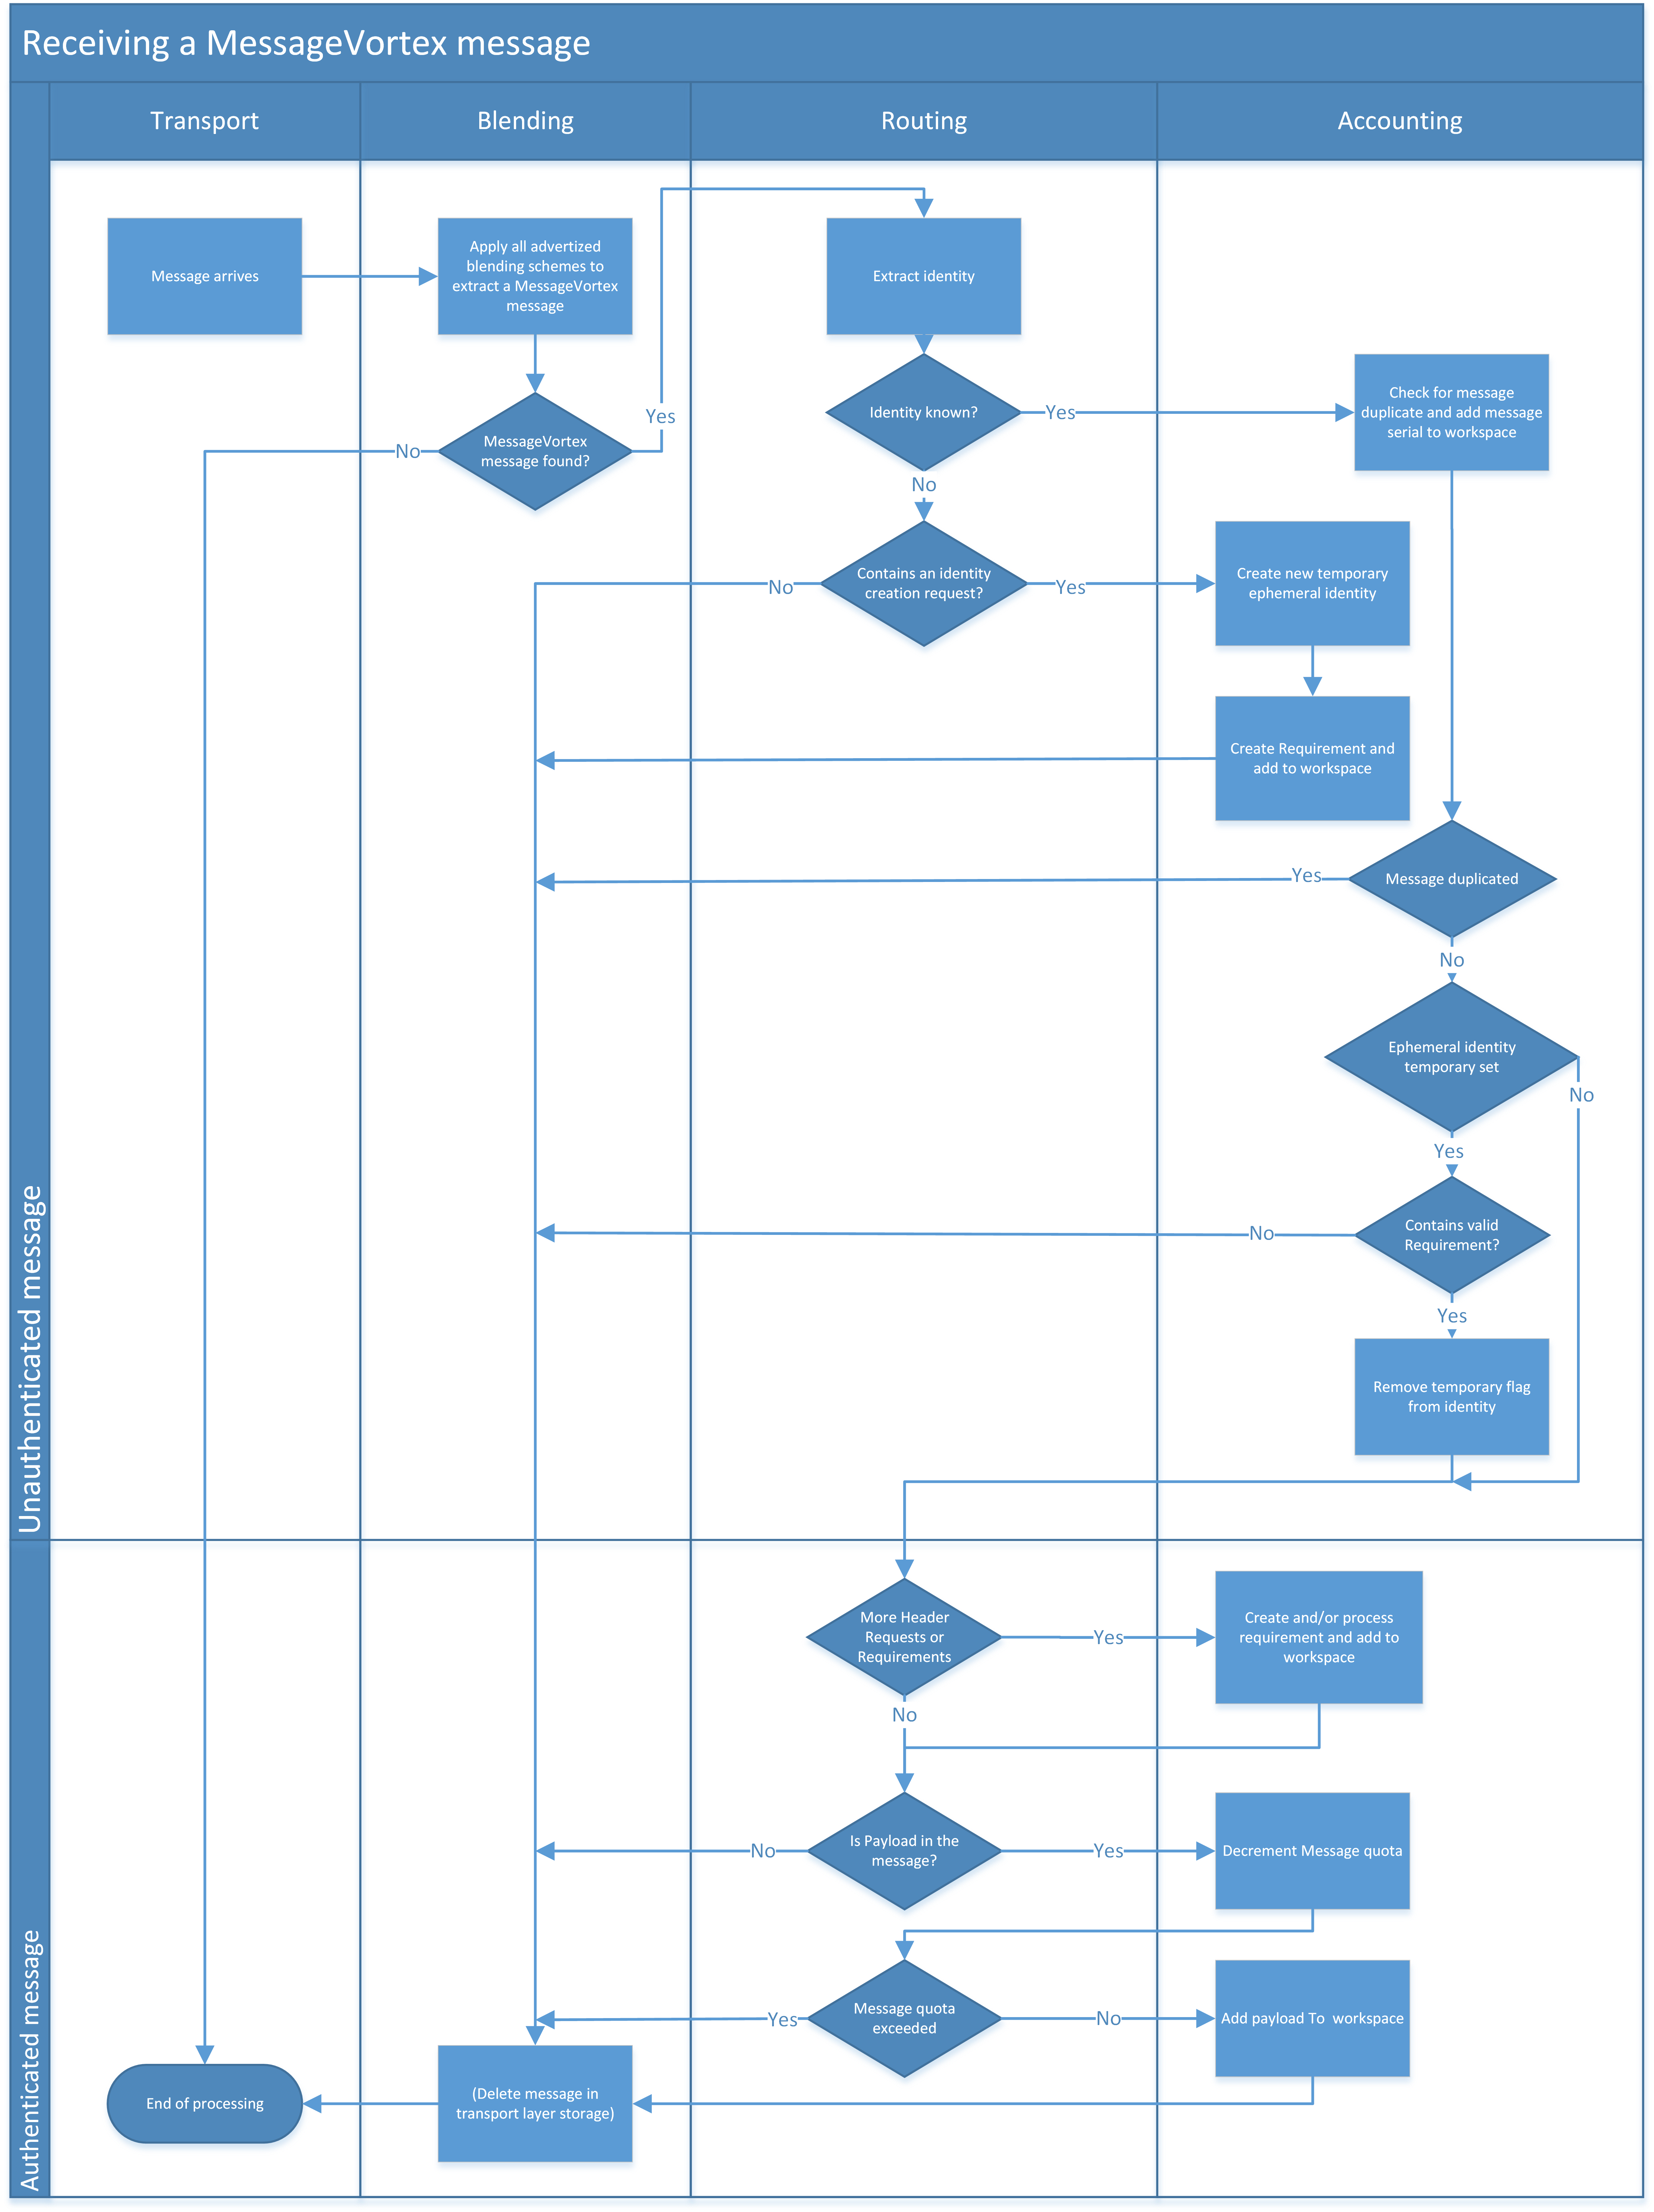
\includegraphics[width=0.90\textwidth]{inc/flowchart_message_receiving}
	\caption{flow diagram showing processing of incomming messages}
	\label{fig:msgRecvProcessing}
\end{figure*}

The processing of a sending block is triggered by a routing block in the workspace, as shown in figure~\ref{fig:msgSendProcessing}. The assembly instructions are processed to collect the payload blocks. Then the encryption is applied to the message and passed on to the blending layer for processing.

\begin{figure*}[hbt]
	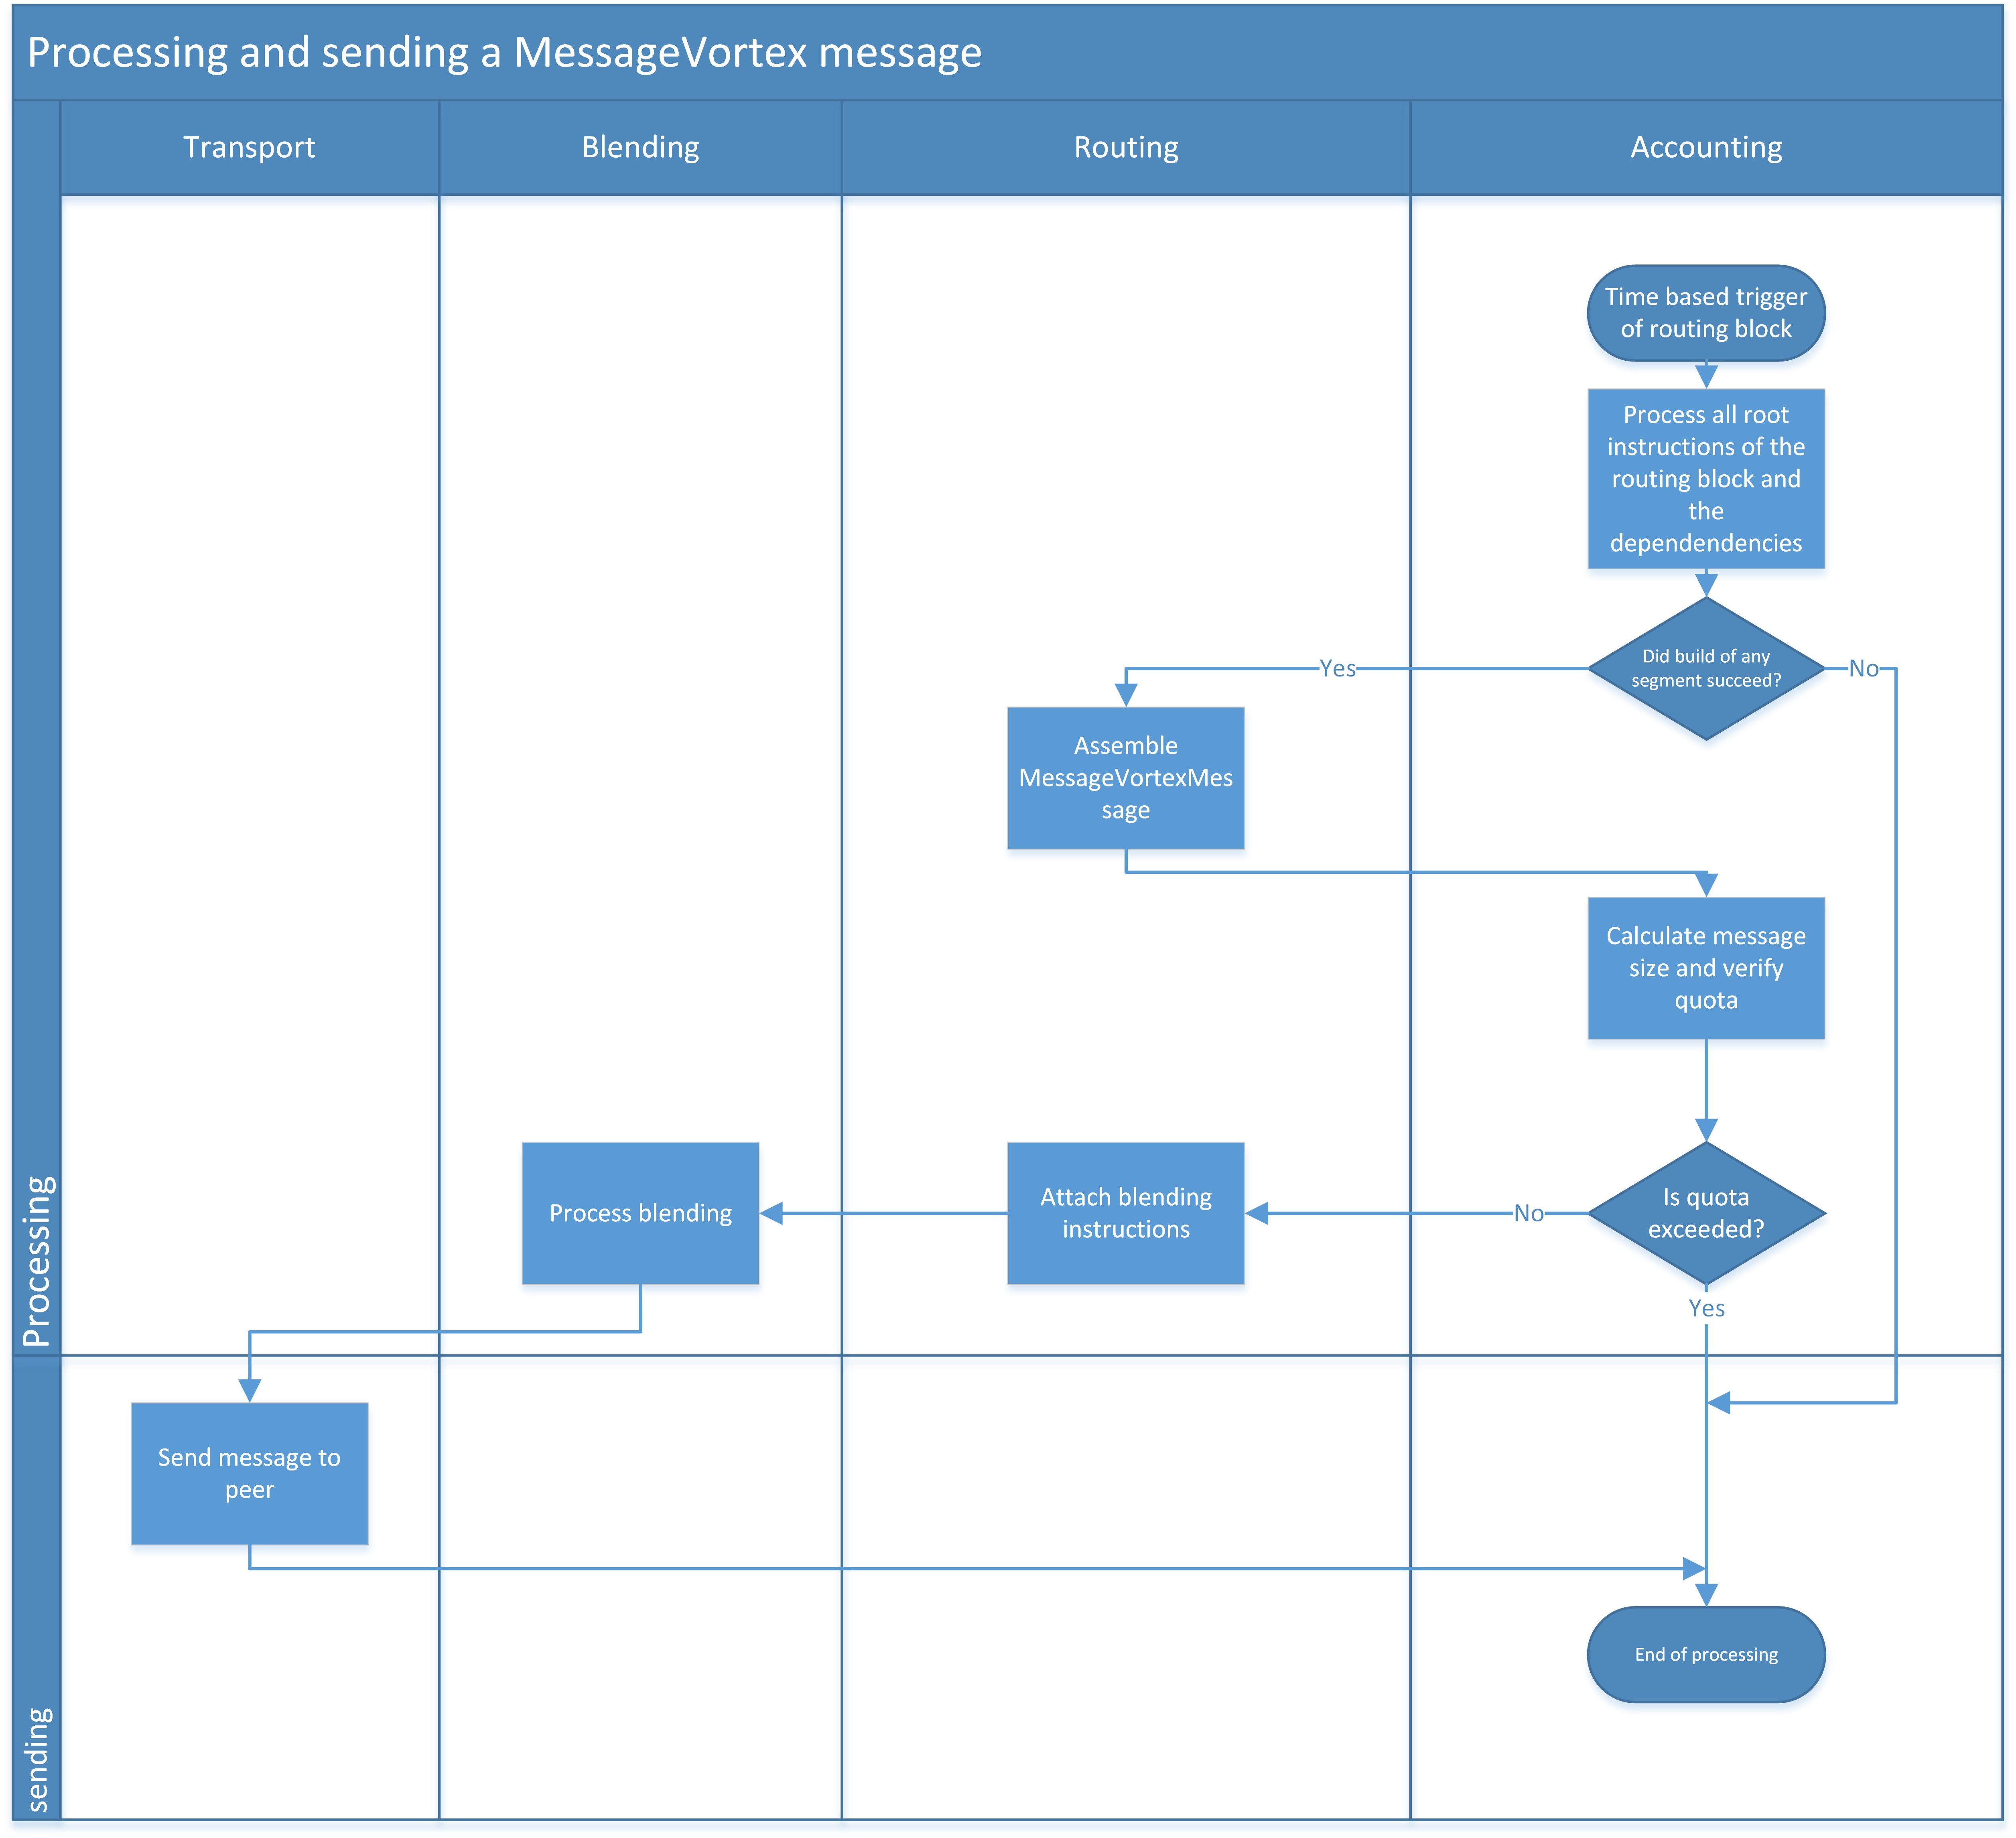
\includegraphics[width=0.90\textwidth]{inc/flowchart_message_sending}
	\caption{flow diagram showing processing of outgoing messages}
	\label{fig:msgSendProcessing}
\end{figure*}

\section{Sub Research Questions Roundup}
We sum up the findings of the last part regarding our three research questions and describe the next steps to be taken.

\subsection{SQ1: Technologies for sending messages maintaining unlinkability against an adversary}
We were unable to identify a single technology that withstands our adversary model entirely. The technologies were either too simple to withstand an adversary (e.g., remailers), have substantial flaws affecting their reliability (e.g., most mixes and DC networks), an active adversary could sabotage them or do not scale.

We were able to describe a rough protocol that performs far better in almost all aspects of anonymity than the solutions described in the previous sections. This comparison was always made for the adversary model given. If we assume that the constraints of trust (only trust in sender and recipient infrastructure, whereas we always have multiple recipients) are valid, we can make the following statements regarding anonymity and unlinkability:
\begin{itemize}
	\item If an adversary identifies all involved nodes of a message and identifies all the corresponding messages and controls, all nodes except for senders and recipients nodes, he can determine message frequency, maximum message size, and message peers.
	\item If an adversary can identify all involved $i$ nodes of a sending party while controlling $j$ nodes, then he may determine a $k$-anonymity set whereas $k=i-j$ for the message set and a maximum message frequency. 
	\item If an adversary is running a node, he may identify other nodes participating in the network by analyzing peer messages.
\end{itemize}

We may safely assume that a carefully crafted message within a standard message flow is therefore unlinked from the two message peers. An adversary running a node may identify over time, possibly participating nodes, but he will be unable to query or use such a node without the corresponding keys. He may be able to observe such nodes, possibly view their activity, but he is unable to match messages generated.

In the next section, we will further elaborate on this protocol and analyze it. We will focus on the question of whether it is possible to create a protocol that withstands threads of the rough modern world.

\subsection{SQ2: Attacking unlinkability and circumvention}
In the previous part, we identified a lot of attack schemes used to attack the anonymity of a protocol or infrastructure. While not all are technical, technicality plays a major part. We identified:
\begin{itemize}
	\item Anonymity attacks
	\begin{itemize}
		\item Hotspot attacks
		\item Side-channel attacks
		\item Sizing analysis
		\item Bugging attacks
		\item Tagging and tracing attacks
		\begin{itemize}
			\item Peer discovering attacks
			\item Traffic flow attacks
		\end{itemize}
	\end{itemize}
	\item Availability and reliability attacks
	\begin{itemize}
		\item Denial of service (DoS) attacks
		\item Censorship attacks
	\end{itemize}
	\item Non-technical Attacks
	\begin{itemize}
		\item Credibility attacks
		\item Censorship attacks
	\end{itemize}
\end{itemize}

We identified several possibilities to circumvent the attack classes listed above. Some of them, such as the bugging attack, may be countered by design (e.g., by allowing only simple messages). Others can only be countered partially in reality (e.g., DDoS attacks). We will further elaborate on the protocol and then analyze the impact of every single attack on the protocol.

\subsection{SQ3: Attack Mitigation by design}
This SQ is a part of the previous question to a certain extent. We identified that reliability and trust are key factors to a protocol. Therefore, allowing a single point of failure (SPOF) or extending trust over central infrastructures is deadly for an anonymizing protocol. 

When elaborating on the protocol in the next part, we will focus on introducing designs that will prohibit actions endangering anonymity. In the Result section, we will focus on all attacks, which should be mitigated by design. 
